\documentclass[a4paper,12pt,twoside]{memoir}

% Castellano
\usepackage[spanish,es-tabla]{babel}
\selectlanguage{spanish}
\usepackage[utf8]{inputenc}
\usepackage[T1]{fontenc}
\usepackage{lmodern} % scalable font
\usepackage{microtype}
\usepackage{placeins}

\RequirePackage{booktabs}
\RequirePackage[table]{xcolor}
\RequirePackage{xtab}
\RequirePackage{multirow}

% Links
\usepackage[colorlinks]{hyperref}
\hypersetup{
	allcolors = {red}
}

% Ecuaciones
\usepackage{amsmath}

% Rutas de fichero / paquete
\newcommand{\ruta}[1]{{\sffamily #1}}

% Párrafos
\nonzeroparskip


% Imagenes
\usepackage{graphicx}
\newcommand{\imagen}[2]{
	\begin{figure}[!h]
		\centering
		\includegraphics[width=0.9\textwidth]{#1}
		\caption{#2}\label{fig:#1}
	\end{figure}
	\FloatBarrier
}

\newcommand{\imagenflotante}[2]{
	\begin{figure}%[!h]
		\centering
		\includegraphics[width=0.9\textwidth]{#1}
		\caption{#2}\label{fig:#1}
	\end{figure}
}



% El comando \figura nos permite insertar figuras comodamente, y utilizando
% siempre el mismo formato. Los parametros son:
% 1 -> Porcentaje del ancho de página que ocupará la figura (de 0 a 1)
% 2 --> Fichero de la imagen
% 3 --> Texto a pie de imagen
% 4 --> Etiqueta (label) para referencias
% 5 --> Opciones que queramos pasarle al \includegraphics
% 6 --> Opciones de posicionamiento a pasarle a \begin{figure}
\newcommand{\figuraConPosicion}[6]{%
  \setlength{\anchoFloat}{#1\textwidth}%
  \addtolength{\anchoFloat}{-4\fboxsep}%
  \setlength{\anchoFigura}{\anchoFloat}%
  \begin{figure}[#6]
    \begin{center}%
      \Ovalbox{%
        \begin{minipage}{\anchoFloat}%
          \begin{center}%
            \includegraphics[width=\anchoFigura,#5]{#2}%
            \caption{#3}%
            \label{#4}%
          \end{center}%
        \end{minipage}
      }%
    \end{center}%
  \end{figure}%
}

%
% Comando para incluir imágenes en formato apaisado (sin marco).
\newcommand{\figuraApaisadaSinMarco}[5]{%
  \begin{figure}%
    \begin{center}%
    \includegraphics[angle=90,height=#1\textheight,#5]{#2}%
    \caption{#3}%
    \label{#4}%
    \end{center}%
  \end{figure}%
}
% Para las tablas
\newcommand{\otoprule}{\midrule [\heavyrulewidth]}
%
% Nuevo comando para tablas pequeñas (menos de una página).
\newcommand{\tablaSmall}[5]{%
 \begin{table}
  \begin{center}
   \rowcolors {2}{gray!35}{}
   \begin{tabular}{#2}
    \toprule
    #4
    \otoprule
    #5
    \bottomrule
   \end{tabular}
   \caption{#1}
   \label{tabla:#3}
  \end{center}
 \end{table}
}

%
%Para el float H de tablaSmallSinColores
\usepackage{float}

%
% Nuevo comando para tablas pequeñas (menos de una página).
\newcommand{\tablaSmallSinColores}[5]{%
 \begin{table}[H]
  \begin{center}
   \begin{tabular}{#2}
    \toprule
    #4
    \otoprule
    #5
    \bottomrule
   \end{tabular}
   \caption{#1}
   \label{tabla:#3}
  \end{center}
 \end{table}
}

\newcommand{\tablaApaisadaSmall}[5]{%
\begin{landscape}
  \begin{table}
   \begin{center}
    \rowcolors {2}{gray!35}{}
    \begin{tabular}{#2}
     \toprule
     #4
     \otoprule
     #5
     \bottomrule
    \end{tabular}
    \caption{#1}
    \label{tabla:#3}
   \end{center}
  \end{table}
\end{landscape}
}

%
% Nuevo comando para tablas grandes con cabecera y filas alternas coloreadas en gris.
\newcommand{\tabla}[6]{%
  \begin{center}
    \tablefirsthead{
      \toprule
      #5
      \otoprule
    }
    \tablehead{
      \multicolumn{#3}{l}{\small\sl continúa desde la página anterior}\\
      \toprule
      #5
      \otoprule
    }
    \tabletail{
      \hline
      \multicolumn{#3}{r}{\small\sl continúa en la página siguiente}\\
    }
    \tablelasttail{
      \hline
    }
    \bottomcaption{#1}
    \rowcolors {2}{gray!35}{}
    \begin{xtabular}{#2}
      #6
      \bottomrule
    \end{xtabular}
    \label{tabla:#4}
  \end{center}
}

%
% Nuevo comando para tablas grandes con cabecera.
\newcommand{\tablaSinColores}[6]{%
  \begin{center}
    \tablefirsthead{
      \toprule
      #5
      \otoprule
    }
    \tablehead{
      \multicolumn{#3}{l}{\small\sl continúa desde la página anterior}\\
      \toprule
      #5
      \otoprule
    }
    \tabletail{
      \hline
      \multicolumn{#3}{r}{\small\sl continúa en la página siguiente}\\
    }
    \tablelasttail{
      \hline
    }
    \bottomcaption{#1}
    \begin{xtabular}{#2}
      #6
      \bottomrule
    \end{xtabular}
    \label{tabla:#4}
  \end{center}
}

%
% Nuevo comando para tablas grandes sin cabecera.
\newcommand{\tablaSinCabecera}[5]{%
  \begin{center}
    \tablefirsthead{
      \toprule
    }
    \tablehead{
      \multicolumn{#3}{l}{\small\sl continúa desde la página anterior}\\
      \hline
    }
    \tabletail{
      \hline
      \multicolumn{#3}{r}{\small\sl continúa en la página siguiente}\\
    }
    \tablelasttail{
      \hline
    }
    \bottomcaption{#1}
  \begin{xtabular}{#2}
    #5
   \bottomrule
  \end{xtabular}
  \label{tabla:#4}
  \end{center}
}



\definecolor{cgoLight}{HTML}{EEEEEE}
\definecolor{cgoExtralight}{HTML}{FFFFFF}

%
% Nuevo comando para tablas grandes sin cabecera.
\newcommand{\tablaSinCabeceraConBandas}[5]{%
  \begin{center}
    \tablefirsthead{
      \toprule
    }
    \tablehead{
      \multicolumn{#3}{l}{\small\sl continúa desde la página anterior}\\
      \hline
    }
    \tabletail{
      \hline
      \multicolumn{#3}{r}{\small\sl continúa en la página siguiente}\\
    }
    \tablelasttail{
      \hline
    }
    \bottomcaption{#1}
    \rowcolors[]{1}{cgoExtralight}{cgoLight}

  \begin{xtabular}{#2}
    #5
   \bottomrule
  \end{xtabular}
  \label{tabla:#4}
  \end{center}
}




\graphicspath{ {./img/} }

% Capítulos
\chapterstyle{bianchi}
\newcommand{\capitulo}[2]{
	\setcounter{chapter}{#1}
	\setcounter{section}{0}
	\chapter*{#2}
	\addcontentsline{toc}{chapter}{#2}
	\markboth{#2}{#2}
}

% Apéndices
\renewcommand{\appendixname}{Apéndice}
\renewcommand*\cftappendixname{\appendixname}

\newcommand{\apendice}[1]{
	%\renewcommand{\thechapter}{A}
	\chapter{#1}
}

\renewcommand*\cftappendixname{\appendixname\ }

% Formato de portada
\makeatletter
\usepackage{xcolor}
\newcommand{\tutor}[1]{\def\@tutor{#1}}
\newcommand{\course}[1]{\def\@course{#1}}
\definecolor{cpardoBox}{HTML}{E6E6FF}
\def\maketitle{
  \null
  \thispagestyle{empty}
  % Cabecera ----------------
\noindent
\includegraphics[width=\textwidth]{cabecera}\vspace{1cm}%
  \vfill
  % Título proyecto y escudo informática ----------------
  \colorbox{cpardoBox}{%
    \begin{minipage}{.8\textwidth}
      \vspace{.5cm}\Large
      \begin{center}
      \textbf{TFG del Grado en Ingeniería Informática}\vspace{.6cm}\\
      \textbf{\LARGE\@title{}}
      \end{center}
      \vspace{.2cm}
    \end{minipage}

  }%
  \hfill\begin{minipage}{.20\textwidth}
    
\includegraphics[width=\textwidth]{escudoInfor}
  \end{minipage}
  \vfill
  % Datos de alumno, curso y tutores ------------------
  \begin{center}%
  {%
    \noindent\LARGE
    Presentado por \@author{}\\ 
    en Universidad de Burgos --- \@date{}\\
    Tutor: \@tutor{}\\
  }%
  \end{center}%
  \null
  \cleardoublepage
  }
\makeatother


% Datos de portada
\title{título del TFG \\Documentación Técnica}
\author{nombre alumno}
\tutor{nombre tutor}
\date{\today}

\begin{document}

\maketitle



\cleardoublepage



%%%%%%%%%%%%%%%%%%%%%%%%%%%%%%%%%%%%%%%%%%%%%%%%%%%%%%%%%%%%%%%%%%%%%%%%%%%%%%%%%%%%%%%%



\frontmatter


\clearpage

% Indices
\tableofcontents

\clearpage

\listoffigures

\clearpage

\listoftables

\clearpage

\mainmatter

\appendix

\apendice{Plan de Proyecto Software}

\section{Introducción}

\section{Planificación temporal}

\section{Estudio de viabilidad}

\subsection{Viabilidad económica}

\subsection{Viabilidad legal}



\apendice{Especificación de Requisitos}

\section{Introducción}

Aunque este trabajo se centra sobre todo en investigación, cuando hablamos de requisitos nos referiremos a los de la aplicación Android generada. En esta sección se enumerarán los requisitos funcionales y no funcionales de la aplicación, y se definirán los casos de uso derivados.  

\section{Objetivos generales}

En la memoria se exponen los objetivos generales del trabajo, los cuales, dada la naturaleza del trabajo, se centran principalmente en la fase de investigación. En este apartado nos centraremos en los requisitos relativos al último de los objetivos generales expuestos: 

<<\textit{Desarrollar una app de Android para mostrar la aplicabilidad del modelo de clasificación generado.}>>

\section{Catalogo de requisitos}

Aquí se enumeran los requisitos funcionales y no funcionales de la aplicación desarrollada para dispositivos Android. Dado que mi compañero de proyecto José Luis Garrido Labrador y yo hemos realizado dos aplicaciones (una web y una para Android) con el mismo objetivo y las mismas funcionalidades, la especificación de los requisitos  se ha realizado de forma conjunta, y por lo tanto, muchos de los puntos de estos apartados coincidirán en ambos trabajos. 

\subsection{Requisitos funcionales}
 
\begin{itemize}
	\item \textbf{RF-1 Confidencialidad del sistema:} Solamente los usuarios autorizados podrán acceder al sistema. 
	
\begin{itemize}
		\item \textbf{RF-1.1 Identificación de usuario:} los usuarios se identificarán con un \textit{nickname} y una contraseña 
		\item \textbf{RF-1.2 Rol de administración:} existirá un usuario especial que podrá administrar el sistema completamente sin restricciones.
		\item \textbf{RF-1.3 Visualización de una cama:} los usuarios validados deben poder observar los datos en tiempo real de las camas disponibles. 
		\item \textbf{RF-1.4 Restricción de acceso:} los usuarios solamente podrán tener acceso a los datos de las camas permitidas. 
		\item \textbf{RF-1.5 Acceso completo al administrador:} el administrador debe poder acceder a los datos de todas las camas existentes.
\end{itemize}
	
	\item \textbf{RF-2 Gestión de las camas:} El administrador debe poder gestionar las camas pudiendo añadir, modificar, borrar y dar acceso a un usuario a los datos de una cama determinada. 
	
\begin{itemize}
		\item \textbf{RF-2.1 Añadir cama:} el administrador debe poder añadir una nueva cama al sistema.
		\item \textbf{RF-2.2 Modificar cama:} el administrador debe poder modificar los datos una cama existente.
		\item \textbf{RF-2.3 Borrar cama:} el administrador debe poder borrar una cama del sistema.
		\item \textbf{RF-2.4 Asignar camas a usuarios:} el administrador se encarga de decidir qué usuario puede acceder a los datos de qué cama.
\end{itemize}
	
	\item \textbf{RF-3 Gestión de los usuarios:} el administrador debe poder gestionar los usuarios pudiendo añadir, modificar y borrar. El usuario debe poder gestionar su propia contraseña. 

\begin{itemize}
		\item \textbf{RF-3.1 Añadir usuario:} el administrador debe poder añadir un nuevo usuario al sistema.
		\item \textbf{RF-3.2 Modificar usuario:} el administrador debe poder modificar los datos un usuario existente. Igualmente el usuario debe poder modificar su propia contraseña. 
		\item \textbf{RF-3.3 Borrar usuario:} el administrador debe poder borrar un usuario del sistema.
\end{itemize}

	\item \textbf{RF-4 Visualización de los datos:} los usuarios deben poder ver, de las camas disponibles, el estado actual del paciente, la probabilidad de crisis epiléptica, sus constantes vitales y las presiones. 
	
\end{itemize}

\subsection{Requisitos no funcionales}

\begin{itemize}
	\item \textbf{RNF-1 Usabilidad:} la aplicación debe cumplir estándares de usabilidad teniendo una curva de aprendizaje baja y un uso de metáforas adecuado.
	\item \textbf{RNF-2 Confidencialidad:} los datos de las camas, al ser en parte constantes vitales de pacientes, solamente han de ser accesibles por los usuarios permitidos.
	\item \textbf{RNF-3 Escalabilidad:} el sistema debe ser escalable para adaptarse de manera correcta a un incremento de carga del sistema.
	\item \textbf{RNF-4 Seguridad:} los usuarios deben poder identificarse sólidamente con el sistema sin que sus datos o sus credenciales (\textit{tokens}) sean accesibles por terceros, incluso el administrador.
\end{itemize}


\section{Especificación de requisitos}

De la misma forma, en lo relativo a las funcionalidades del cliente, la especificación de los casos de uso se ha hecho de forma conjunta con mi compañero José Luis Garrido Labrador, por lo que los contenidos de este apartado coincidirán en gran medida con los suyos. 

\subsection{Actores}

En los casos de uso se distinguen dos actores: 
\begin{itemize}
	\item \textbf{Administrador:} Tiene acceso a la gestión de usuarios, la gestión de camas y la visualización de los datos de todas las camas existentes. 
	\item \textbf{Usuario:} Tiene acceso a la visualización de los datos de las camas que tiene asignadas y a la gestión de su propio usuario. 
\end{itemize}

\subsection{Diagramas de casos de uso}

\begin{figure}[H]
	\centering
	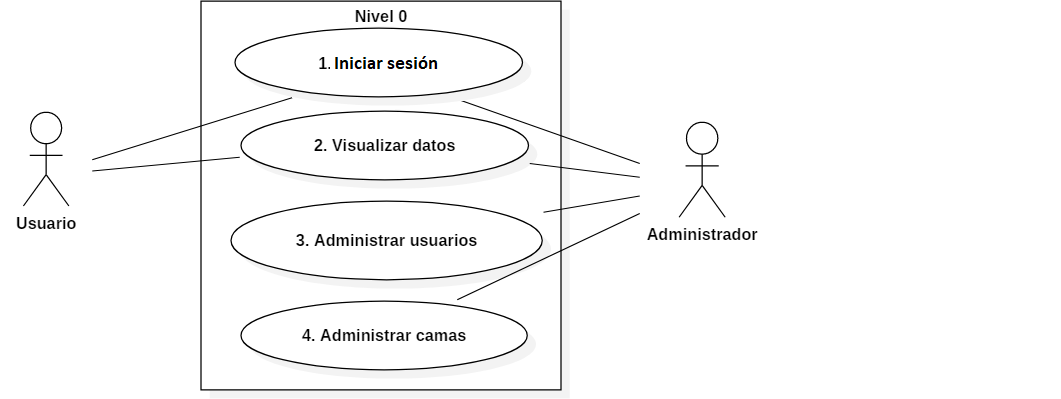
\includegraphics[width=1\textwidth]{../img/cu-n0.png}
	\caption{Diagrama de casos de uso, nivel 0.}
	\label{fig:cu-n0}
\end{figure}

\begin{figure}[H]
	\centering
	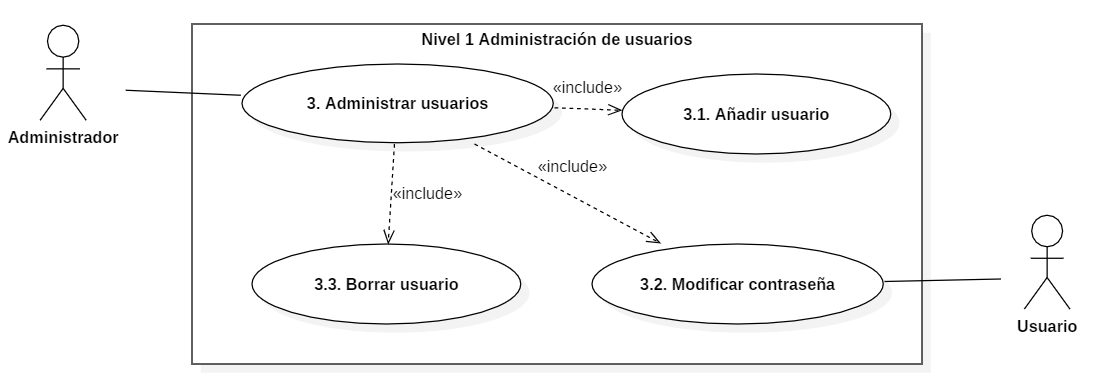
\includegraphics[width=1\textwidth]{../img/cu-n1-2.png}
	\caption{Diagrama de casos de uso, visualización de datos.}
	\label{fig:cu-n1.2}
\end{figure}

\begin{figure}[H]
	\centering
	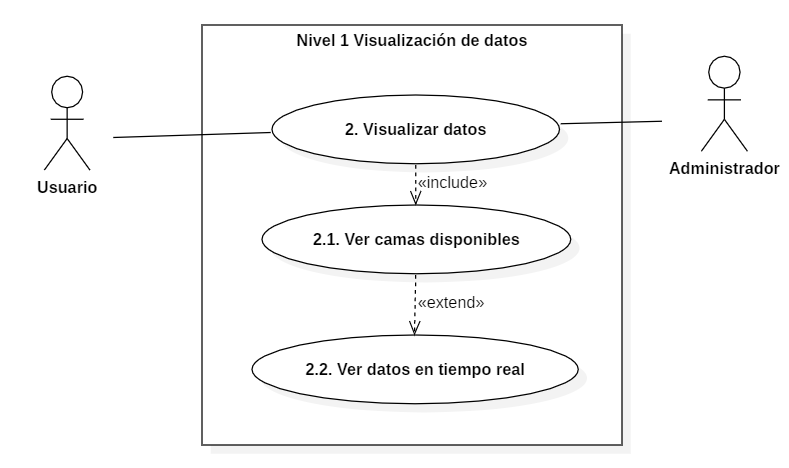
\includegraphics[width=1\textwidth]{../img/cu-n1-3.png}
	\caption{Diagrama de casos de uso, administración de usuarios.}
	\label{fig:cu-n1.3}
\end{figure}

\begin{figure}[H]
	\centering
	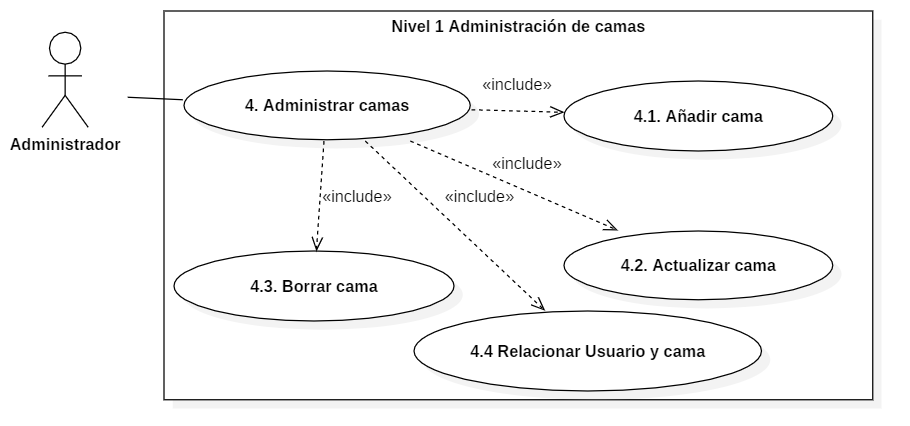
\includegraphics[width=1\textwidth]{../img/cu-n1-4.png}
	\caption{Diagrama de casos de uso, administración de camas.}
	\label{fig:cu-n1.4}
\end{figure}

\subsection{Especificación de casos de uso}

\tablaSmallSinColores{Caso de uso 1: Iniciar sesión }{p{3cm} p{.75cm} p{9cm}}{tablaCU1}{
	\multicolumn{3}{p{10.25cm}}{CU-1: Iniciar sesión} \\
}
{
	Descripción                            & \multicolumn{2}{p{10.25cm}}{El usuario se identifica en el sistema} \\\hubu
	Precondiciones                         & \multicolumn{2}{p{10.25cm}}{No existe una sesión activa válida} \\\hubu
	Requisitos                         	   & \multicolumn{2}{p{10.25cm}}{RF-1, RF-1.1} \\\hubu
	Usuario                         	   & \multicolumn{2}{p{10.25cm}}{Anónimo} \\\hubu
	\multirow{3}{3.5cm}{Secuencia normal}  & Paso & Acción \\\cline{2-3}
	& 1    & El cliente envía sus credenciales al servidor \\\cline{2-3}
	& 2    & El servidor acepta las credenciales devolviendo el token de sesión \\\hubu
	Postcondiciones                        & \multicolumn{2}{p{10.25cm}}{El usuario tiene una sesión activa válida} \\\hubu
	\multirow{2}{3.5cm}{Excepciones}       & Paso & Acción \\\cline{2-3}
	& 2    & Si las credenciales son incorrectas el servidor responde con error \\\hubu
	Frecuencia                             & Alta \\\hubu
	Importancia                            & Crítico \\\hubu
	Comentarios                            & \multicolumn{2}{p{10.25cm}}{Es siempre lo primero que aparecerá} \\
}

\tablaSmallSinColores{Caso de uso 2: Visualizar de datos }{p{3cm} p{.75cm} p{9cm}}{tablaCU2}{
	\multicolumn{3}{p{10.25cm}}{CU-2: Visualizar de datos} \\
}
{
	Descripción                            & \multicolumn{2}{p{10.25cm}}{Ver lista de las camas disponibles} \\\hubu
	Precondiciones                         & \multicolumn{2}{p{10.25cm}}{Sesión activa válida} \\\hubu
	Requisitos                         	   & \multicolumn{2}{p{10.25cm}}{RF-1.3, RF-1.4} \\\hubu
	Usuario                         	   & \multicolumn{2}{p{10.25cm}}{Administrador y Usuario} \\\hubu
	\multirow{3}{3.5cm}{Secuencia normal}  & Paso & Acción \\\cline{2-3}
	& 1    & El cliente solicita ver las camas disponibles \\\hubu
	Postcondiciones                        & \multicolumn{2}{p{10.25cm}}{El cliente está en la pantalla de camas disponibles} \\\hubu
	Frecuencia                             & Alta \\\hubu
	Importancia                            & Alta \\
}

\tablaSmallSinColores{Caso de uso 2.1: Elegir cama }{p{3cm} p{.75cm} p{9cm}}{tablaCU21}{
	\multicolumn{3}{p{10.25cm}}{CU-2.1: Elegir cama} \\
}
{
	Descripción                            & \multicolumn{2}{p{10.25cm}}{Elegir cama} \\\hubu
	Precondiciones                         & \multicolumn{2}{p{10.25cm}}{Sesión activa válida} \\\hubu
	Requisitos                         	   & \multicolumn{2}{p{10.25cm}}{RF-1.3, RF-1.4, RF-4} \\\hubu
	Usuario                         	   & \multicolumn{2}{p{10.25cm}}{Logueado} \\\hubu
	\multirow{3}{3.5cm}{Secuencia normal}  & Paso & Acción \\\cline{2-3}
	& 1    & El cliente solicita ver las camas disponibles \\\cline{2-3}
	& 2    & El servidor abre conexiones paralelas para actualizar en tiempo real el estado de las camas \\\cline{2-3}
	& 3    & El cliente decide que cama ver \\\hubu
	Postcondiciones                        & \multicolumn{2}{p{10.25cm}}{El cliente entra en la ventana de los datos en tiempo real} \\\hubu
	Frecuencia                             & Alta \\\hubu
	Importancia                            & Alta \\
}

\tablaSmallSinColores{Caso de uso 2.2: Ver datos en tiempo real }{p{3cm} p{.75cm} p{9cm}}{tablaCU22}{
	\multicolumn{3}{p{10.25cm}}{CU-2.2: Ver datos en tiempo real} \\
}
{
	Descripción                            & \multicolumn{2}{p{10.25cm}}{Ver datos en tiempo real} \\\hubu
	Precondiciones                         & \multicolumn{2}{p{10.25cm}}{Sesión activa válida y cama existente y accesible} \\\hubu
	Requisitos                         	   & \multicolumn{2}{p{10.25cm}}{RF-1.3, RF-1.4, RF-4} \\\hubu
	Usuario                         	   & \multicolumn{2}{p{10.25cm}}{Administrador y usuario} \\\hubu
	\multirow{3}{3.5cm}{Secuencia normal}  & Paso & Acción \\\cline{2-3}
	& 1    & El cliente solicita una nueva conexión \\\cline{2-3}
	& 2    & El servidor provee una conexión en tiempo real con los datos \\\hubu
	Postcondiciones                        & \multicolumn{2}{p{10.25cm}}{El usuario tiene una conexión paralela abierta con los datos en tiempo real} \\\hubu
	\multirow{2}{3.5cm}{Excepciones}       & Paso & Acción \\\cline{2-3}
	& 2    & Si un paquete faltase o la señal fuera, débil se alertaría al usuario \\\hubu
	Frecuencia                             & Alta \\\hubu
	Importancia                            & Máxima \\}

\tablaSmallSinColores{Caso de uso 3: Administrar de usuarios }{p{3cm} p{.75cm} p{9cm}}{tablaCU3}{
	\multicolumn{3}{p{10.25cm}}{CU-3: Administrar de usuarios} \\
}
{
	Descripción                            & \multicolumn{2}{p{10.25cm}}{Administración de usuario: alta, baja y modificación} \\\hubu
	Precondiciones                         & \multicolumn{2}{p{10.25cm}}{Sesión de administrador válida} \\\hubu
	Requisitos                         	   & \multicolumn{2}{p{10.25cm}}{RF-3} \\\hubu
	Usuario                         	   & \multicolumn{2}{p{10.25cm}}{Administrador} \\\hubu
	\multirow{3}{3.5cm}{Secuencia normal}  & Paso & Acción \\\cline{2-3}
	& 1    & El administrador entra en el menú de administración de usuarios \\\hubu
	Postcondiciones                        & \multicolumn{2}{p{10.25cm}}{El administrador está en el menú de administración de usuarios} \\\hubu
	Frecuencia                             & Baja \\\hubu
	Importancia                            & Alta \\
}

\tablaSmallSinColores{Caso de uso 3.1: Añadir usuarios }{p{3cm} p{.75cm} p{9cm}}{tablaCU31}{
	\multicolumn{3}{p{10.25cm}}{CU-3.1: Añadir usuarios} \\
}
{
	Descripción                            & \multicolumn{2}{p{10.25cm}}{Añadir usuarios} \\\hubu
	Precondiciones                         & \multicolumn{2}{p{10.25cm}}{Sesión de administración activa} \\\hubu
	Requisitos                         	   & \multicolumn{2}{p{10.25cm}}{RF-3.1} \\\hubu
	Usuario                         	   & \multicolumn{2}{p{10.25cm}}{Administrador} \\\hubu
	\multirow{3}{3.5cm}{Secuencia normal}  & Paso & Acción \\\cline{2-3}
	& 1    & El administrador elige añadir un nuevo usuario \\\cline{2-3}
	& 2    & Se introduce un nombre de usuario para identificarlo \\\cline{2-3}
	& 3    & Se introduce una contraseña dos veces \\\cline{2-3}
	& 4    & Se almacenan los datos \\\hubu
	Postcondiciones                        & \multicolumn{2}{p{10.25cm}}{Existe un nuevo usuario en el sistema} \\\hubu
	\multirow{2}{3.5cm}{Excepciones}       & Paso & Acción \\\cline{2-3}
	& 2    & Si el nickname existiese \\\cline{2-3}
	& 3    & La contraseña añadida no coincide en las dos ocasiones \\\hubu
	Frecuencia                             & Baja \\\hubu
	Importancia                            & Alta \\
}

\tablaSmallSinColores{Caso de uso 3.2: Modificar contraseña }{p{3cm} p{.75cm} p{9cm}}{tablaCU32}{
	\multicolumn{3}{p{10.25cm}}{CU-3.2: Modificar contraseña} \\
}
{
	Descripción                            & \multicolumn{2}{p{10.25cm}}{Cambiar la contraseña de un usuario} \\\hubu
	Precondiciones                         & \multicolumn{2}{p{10.25cm}}{Sesión activa válida, usuario existente} \\\hubu
	Requisitos                         	   & \multicolumn{2}{p{10.25cm}}{RF-3.2} \\\hubu
	Usuario                         	   & \multicolumn{2}{p{10.25cm}}{Administrador y Usuario} \\\hubu
	\multirow{3}{3.5cm}{Secuencia normal}  & Paso & Acción \\\cline{2-3}
	& 1    & Si es usuario genérico ir a 3 \\\cline{2-3}
	& 2    & Si es administrador elegir a qué usuario cambiar la contraseña \\\cline{2-3}
	& 3    & Se introduce una contraseña nueva dos veces \\\cline{2-3}
	& 4    & Se actualizan los datos \\\hubu
	Postcondiciones                        & \multicolumn{2}{p{10.25cm}}{La contraseña ha cambiado} \\\hubu
	\multirow{2}{3.5cm}{Excepciones}       & Paso & Acción \\\cline{2-3}
	& 3    & La contraseña añadida no coincide en las dos ocasiones \\\hubu
	Frecuencia                             & Baja \\\hubu
	Importancia                            & Alta \\
}

\tablaSmallSinColores{Caso de uso 3.3: Borrar usuario }{p{3cm} p{.75cm} p{9cm}}{tablaCU33}{
	\multicolumn{3}{p{10.25cm}}{CU-3.3: Borrar usuario} \\
}
{
	Descripción                            & \multicolumn{2}{p{10.25cm}}{Elimina un usuario de la base de datos} \\\hubu
	Precondiciones                         & \multicolumn{2}{p{10.25cm}}{Sesión de administración válida, usuario existente} \\\hubu
	Requisitos                         	   & \multicolumn{2}{p{10.25cm}}{RF-3.3} \\\hubu
	Usuario                         	   & \multicolumn{2}{p{10.25cm}}{Administrador} \\\hubu
	\multirow{3}{3.5cm}{Secuencia normal}  & Paso & Acción \\\cline{2-3}
	& 1    & Elegir a que usuario (no administrador) eliminar \\\cline{2-3}
	& 2    & Eliminar usuario y todos los datos vinculados \\\hubu
	Postcondiciones                        & \multicolumn{2}{p{10.25cm}}{El usuario ha sido eliminado} \\\hubu
	Frecuencia                             & Baja \\\hubu
	Importancia                            & Media \\
}

\tablaSmallSinColores{Caso de uso 4: Administrar de camas }{p{3cm} p{.75cm} p{9cm}}{tablaCU4}{
	\multicolumn{3}{p{10.25cm}}{CU-4: Administrar de camas} \\
}
{
	Descripción                            & \multicolumn{2}{p{10.25cm}}{Administración de camas: alta, baja, modificación y asignación a usuarios} \\\hubu
	Precondiciones                         & \multicolumn{2}{p{10.25cm}}{Sesión de administración válida} \\\hubu
	Requisitos                         	   & \multicolumn{2}{p{10.25cm}}{RF-2} \\\hubu
	Usuario                         	   & \multicolumn{2}{p{10.25cm}}{Administrador} \\\hubu
	\multirow{3}{3.5cm}{Secuencia normal}  & Paso & Acción \\\cline{2-3}
	& 1    & El administrador entra en el menú de administración de camas \\\hubu
	Postcondiciones                        & \multicolumn{2}{p{10.25cm}}{El administrador está en el menú de administración de camas} \\\hubu
	Frecuencia                             & Baja \\\hubu
	Importancia                            & Media \\
}

\tablaSmallSinColores{Caso de uso 4.1: Añadir cama }{p{3cm} p{.75cm} p{9cm}}{tablaCU41}{
	\multicolumn{3}{p{10.25cm}}{CU-4.1: Añadir cama} \\
}
{
	Descripción                            & \multicolumn{2}{p{10.25cm}}{Añadir cama} \\\hubu
	Precondiciones                         & \multicolumn{2}{p{10.25cm}}{Sesión de administración válida} \\\hubu
	Requisitos                         	   & \multicolumn{2}{p{10.25cm}}{RF-2.1} \\\hubu
	Usuario                         	   & \multicolumn{2}{p{10.25cm}}{Administrador} \\\hubu
	\multirow{3}{3.5cm}{Secuencia normal}  & Paso & Acción \\\cline{2-3}
	& 1    & El administrador elige añadir una nueva cama \\\cline{2-3}
	& 2    & Se introduce el grupo multicast de la cama (IP y Puerto) \\\cline{2-3}
	& 3    & Se introduce el nombre identificador\\\cline{2-3}
	& 4    & Se almacenan los datos \\\hubu
	Postcondiciones                        & \multicolumn{2}{p{10.25cm}}{Existe una nueva cama en el sistema} \\\hubu
	\multirow{2}{3.5cm}{Excepciones}       & Paso & Acción \\\cline{2-3}
	& 2    & El grupo multicast pertenece a otra cama \\\cline{2-3}
	& 3    & El nombre identificativo existe para otra cama \\\hubu
	Frecuencia                             & Media \\\hubu
	Importancia                            & Crítica \\\hubu
	Comentarios                            & \multicolumn{2}{p{10.25cm}}{El grupo multicast se configura en la cama y el administrador solamente debe conocerlo, no configurar la cama física} \\
}

\tablaSmallSinColores{Caso de uso 4.2: Modificar cama }{p{3cm} p{.75cm} p{9cm}}{tablaCU42}{
	\multicolumn{3}{p{10.25cm}}{CU-2.2: Modificar cama} \\
}
{
	Descripción                            & \multicolumn{2}{p{10.25cm}}{Modificar los datos de la cama} \\\hubu
	Precondiciones                         & \multicolumn{2}{p{10.25cm}}{Sesión de administración válida, cama existente} \\\hubu
	Requisitos                         	   & \multicolumn{2}{p{10.25cm}}{RF-2.2} \\\hubu
	Usuario                         	   & \multicolumn{2}{p{10.25cm}}{Administrador} \\\hubu
	\multirow{3}{3.5cm}{Secuencia normal}  & Paso & Acción \\\cline{2-3}
	& 1    & Se elige que cama modificar \\\cline{2-3}
	& 2    & Se actualizan los datos a conveniencia del administrador según CU-4.1\\\cline{2-3}
	& 4    & Se actualizan los datos \\\hubu
	Postcondiciones                        & \multicolumn{2}{p{10.25cm}}{Los datos de la cama se modifican} \\\hubu
	\multirow{2}{3.5cm}{Excepciones}       & Paso & Acción \\\cline{2-3}
	& 2    & Mismas excepciones que en CU-4.1 \\\hubu
	Frecuencia                             & Baja \\\hubu
	Importancia                            & Alta \\
}

\tablaSmallSinColores{Caso de uso 4.3: Borrar cama }{p{3cm} p{.75cm} p{9cm}}{tablaCU43}{
	\multicolumn{3}{p{10.25cm}}{CU-4.3: Borrar cama} \\
}
{
	Descripción                            & \multicolumn{2}{p{10.25cm}}{Elimina una cama de la base de datos} \\\hubu
	Precondiciones                         & \multicolumn{2}{p{10.25cm}}{Sesión de administrador válida, cama existente} \\\hubu
	Requisitos                         	   & \multicolumn{2}{p{10.25cm}}{RF-2.3} \\\hubu
	Usuario                         	   & \multicolumn{2}{p{10.25cm}}{Administrador} \\\hubu
	\multirow{3}{3.5cm}{Secuencia normal}  & Paso & Acción \\\cline{2-3}
	& 1    & Elegir a que cama eliminar \\\cline{2-3}
	& 2    & Eliminar cama y todos los datos vinculados \\\hubu
	Postcondiciones                        & \multicolumn{2}{p{10.25cm}}{La cama ya no está en la base de datos} \\\hubu
	Frecuencia                             & Baja \\\hubu
	Importancia                            & Media \\
}

\tablaSmallSinColores{Caso de uso 4.4: Asignar cama a usuario }{p{3cm} p{.75cm} p{9cm}}{tablaCU44}{
	\multicolumn{3}{p{10.25cm}}{CU-4.4: Asignar cama a usuario} \\
}
{
	Descripción                            & \multicolumn{2}{p{10.25cm}}{Permite a un usuario ver los datos de una cama o quitar ese permiso} \\\hubu
	Precondiciones                         & \multicolumn{2}{p{10.25cm}}{Sesión de administración válida, cama y usuario existentes} \\\hubu
	Requisitos                         	   & \multicolumn{2}{p{10.25cm}}{RF-2.4} \\\hubu
	Usuario                         	   & \multicolumn{2}{p{10.25cm}}{Administrador} \\\hubu
	\multirow{3}{3.5cm}{Secuencia normal}  & Paso & Acción \\\cline{2-3}
	& 1    & Elegir cama \\\cline{2-3}
	& 2    & Elegir usuario \\\cline{2-3}
	& 3    & Si la relación existe se puede eliminar el permiso \\\cline{2-3}
	& 3    & Si la relación no existe se puede crear el permiso \\\hubu
	Postcondiciones                        & \multicolumn{2}{p{10.25cm}}{El usuario tiene acceso a la cama, o pierde el mismo} \\\hubu
	Frecuencia                             & Media \\\hubu
	Importancia                            & Crítica \\
}




\apendice{Especificación de diseño}

\section{Introducción}
En esta sección se va a hablar de los aspectos más relevantes del diseño de la aplicación de Android.
\begin{itemize}
	\item En primer lugar, se hará una breve mención al diseño de los datos.
	\item A continuación, en el apartado de diseño procedimental se expondrán detalladamente los dos procesos más relevantes de la aplicación, y en los que se basa fundamentalmente su comportamiento, obviando otros procesos más sencillos o basados en objetos propios del \textit{framework} de Android cuyo funcionamiento puede encontrarse en la documentación.
	\item Después se expondrán las características de la arquitectura general de la aplicación, considerando dos puntos de vista que pueden servir para definir de forma complementaria la arquitectura general del sistema. 
	\item Por último se expondrán los prototipos de la interfaz de usuario generados antes del desarrollo de la aplicación. 
\end{itemize}

\section{Diseño de datos}

Para el desarrollo de la aplicación Android no podemos hablar estrictamente de un diseño de los datos, ya que se trata de un cliente que no interactúa directamente con la base de datos. El acceso a la persistencia se hace a través de peticiones a la API del servidor, la cual devuelve siempre todos los datos en un objeto con formato JSON. 

En este sentido, podemos abstraernos del diseño e implementación concretos de la base de datos, ya que nuestra gestión de los datos solo depende de las características del JSON que nos va a devolver cada petición. La estructura de la respuesta de cada petición a la API se especifica en el Manual del programador de mi compañero José Luis Garrido Labrador. 

\section{Diseño procedimental}

Como se explica más adelante, el funcionamiento general de la aplicación se basa en la comunicación con la API del servidor remoto, el cual proporciona el modelo de datos y la lógica de negocio. Por esta razón, los procesos más relevantes corresponden con los que permiten realizar la comunicación de la aplicación con la API del servidor remoto. 

Tal y como se ha planteado la aplicación de Android, existen dos procesos relevantes que es importante entender, ya que supondrán la base del funcionamiento de la aplicación:

\begin{itemize}
	\item En primer lugar, la \textbf{llamada a los servicios genéricos de la API}. Todas las interacciones con la lógica de negocio de la aplicación (iniciar sesión, visualizar usuarios, añadir usuarios...) se realizan de esta manera. Por esta razón, para garantizar el buen funcionamiento de la aplicación, este proceso debe incluir una comprobación sobre si existe conexión a internet, si la sesión está activa y si la respuesta de la API es la esperada.
	
	Esta interacción se representa en el diagrama de secuencias de la figura~\ref{fig:sequenceAPI}. El elemento \textit{Activity} corresponde con cualquiera de las clases que extienden de \textit{AppCompatActivity} desde las que se realiza una petición a la API del servidor. 
	
	\item En segundo lugar, \textbf{la petición y recepción de los datos de una cama en tiempo real}. Este proceso se realiza a través de conexión a nivel de \textit{sockets} con el servidor y la gestión de eventos empleando la librería Socket.IO. 
	
	Esta interacción se representa en el diagrama de secuencias de la figura~\ref{fig:sequenceStreaming}. Los mensajes \texttt{give\_me\_data} y \texttt{package} son eventos de Socket.IO definidos por el programador de la API. 
\end{itemize}

\begin{figure}[H]
	\centering
	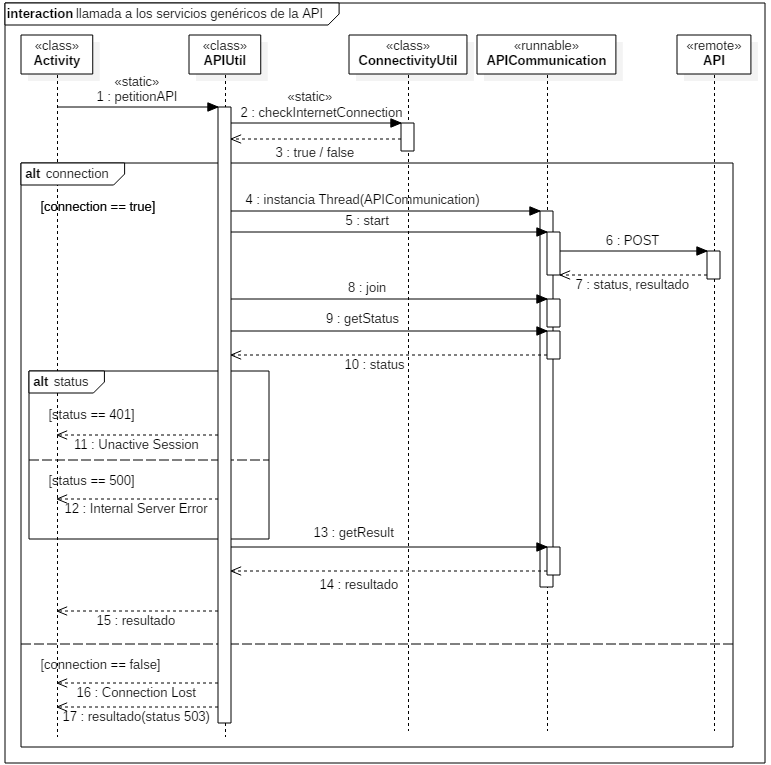
\includegraphics[width=1\textwidth]{../img/sequenceAPI.png}
	\caption{Diagrama de secuencias, llamada a los servicios genéricos de la API.}
	\label{fig:sequenceAPI}
\end{figure}

\begin{figure}[H]
	\centering
	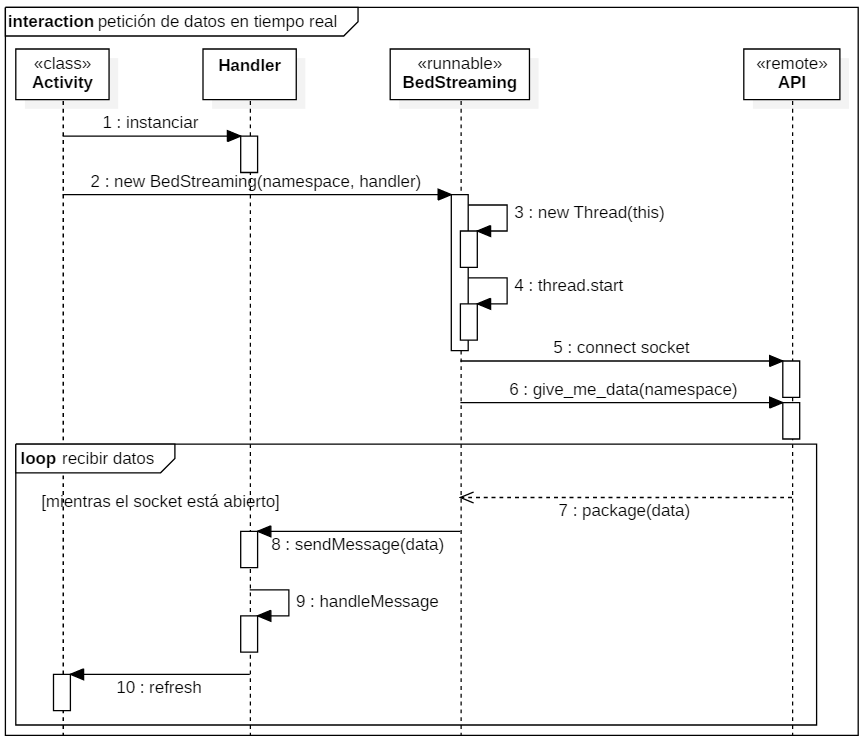
\includegraphics[width=1\textwidth]{../img/sequenceStreaming.png}
	\caption{Diagrama de secuencias, petición de datos en tiempo real.}
	\label{fig:sequenceStreaming}
\end{figure}

El funcionamiento del resto de procesos es fácilmente deducible a partir del código o corresponde con el uso de elementos propios del \textit{framework} de Android. La especificación y funcionamiento de estos elementos se puede consultar en la página web oficial de \textit{Android Developers}~\cite{androiddevelopers}.  

\section{Diseño arquitectónico}

La arquitectura de la aplicación puede verse desde varios puntos de vista. En el contexto del patrón arquitectónico Modelo-Vista-Controlador (MVC)~\cite{wiki:mvc} definimos tres componentes: 
\begin{itemize}
	\item \textbf{Modelo:} Contiene la estructura de los datos que maneja el programa e interactúa con la persistencia para realizar consultas y actualizaciones. 
	\item \textbf{Vista:} Presenta los datos del modelo y la interacción con la lógica de negocio de forma adecuada para el usuario. 
	\item \textbf{Controlador:} Responde a eventos generados por la interacción del usuario con la vista y realiza peticiones de consulta/actualización al modelo. Se puede ver como un intermediario entre ambos componentes. 
\end{itemize}

Según la definición de los componentes de este patrón, la aplicación Android podría ser considerada únicamente como un componente <<Vista>> de un sistema más grande formado también por los los servicios proporcionados por la API del servidor remoto, la cual proporciona el acceso a la persistencia y la comunicación entre el modelo de datos y la aplicación. 

Por otro lado, cuando se habla de este tipo de aplicaciones, es común encontrarnos con el término \textbf{<<arquitectura de microservicios>>}. Según esta arquitectura, cada funcionalidad se encuentra contenida en un proceso del servidor al que llamaremos microservicio. Cada microservicio encapsula un solo aspecto de la lógica de negocio, y los microservicios son procesos independientes entre sí. Tal y como ocurre en esta aplicación Android, el cliente se limita a hacer peticiones a los microservicios de la API del servidor remoto, los cuales, basándose en la lógica de negocio, le proporcionan los datos necesarios para actualizar la <<vista>> o interfaz de usuario. 

\begin{figure}[H]
	\centering
	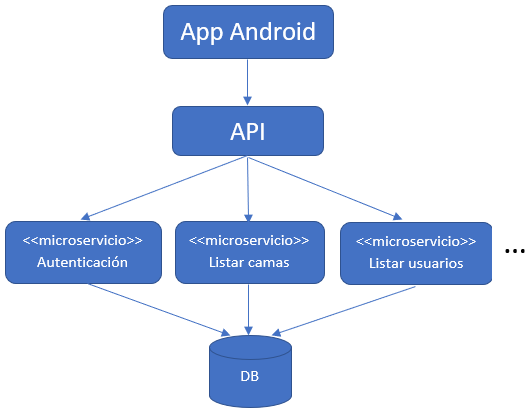
\includegraphics[width=0.8\textwidth]{../img/microservicios.png}
	\caption{Abstracción de la arquitectura de microservicios.}
	\label{fig:microservicios}
\end{figure}

\section{Diseño de interfaces}

Inicialmente se realizaron una serie de prototipos básicos en los que se plasmaron las principales funcionalidades de la aplicación, sin prestar especial atención a los aspectos estéticos de la misma. Para ello se usó la herramienta de prototipado Pencil, ya que permite incorporar elementos propios de la guía de estilos que se ha seguido para el diseño de las interfaces de usuario: \textit{Material Design}~\cite{materialdesign}. 

\begin{figure}[H]
	\centering
	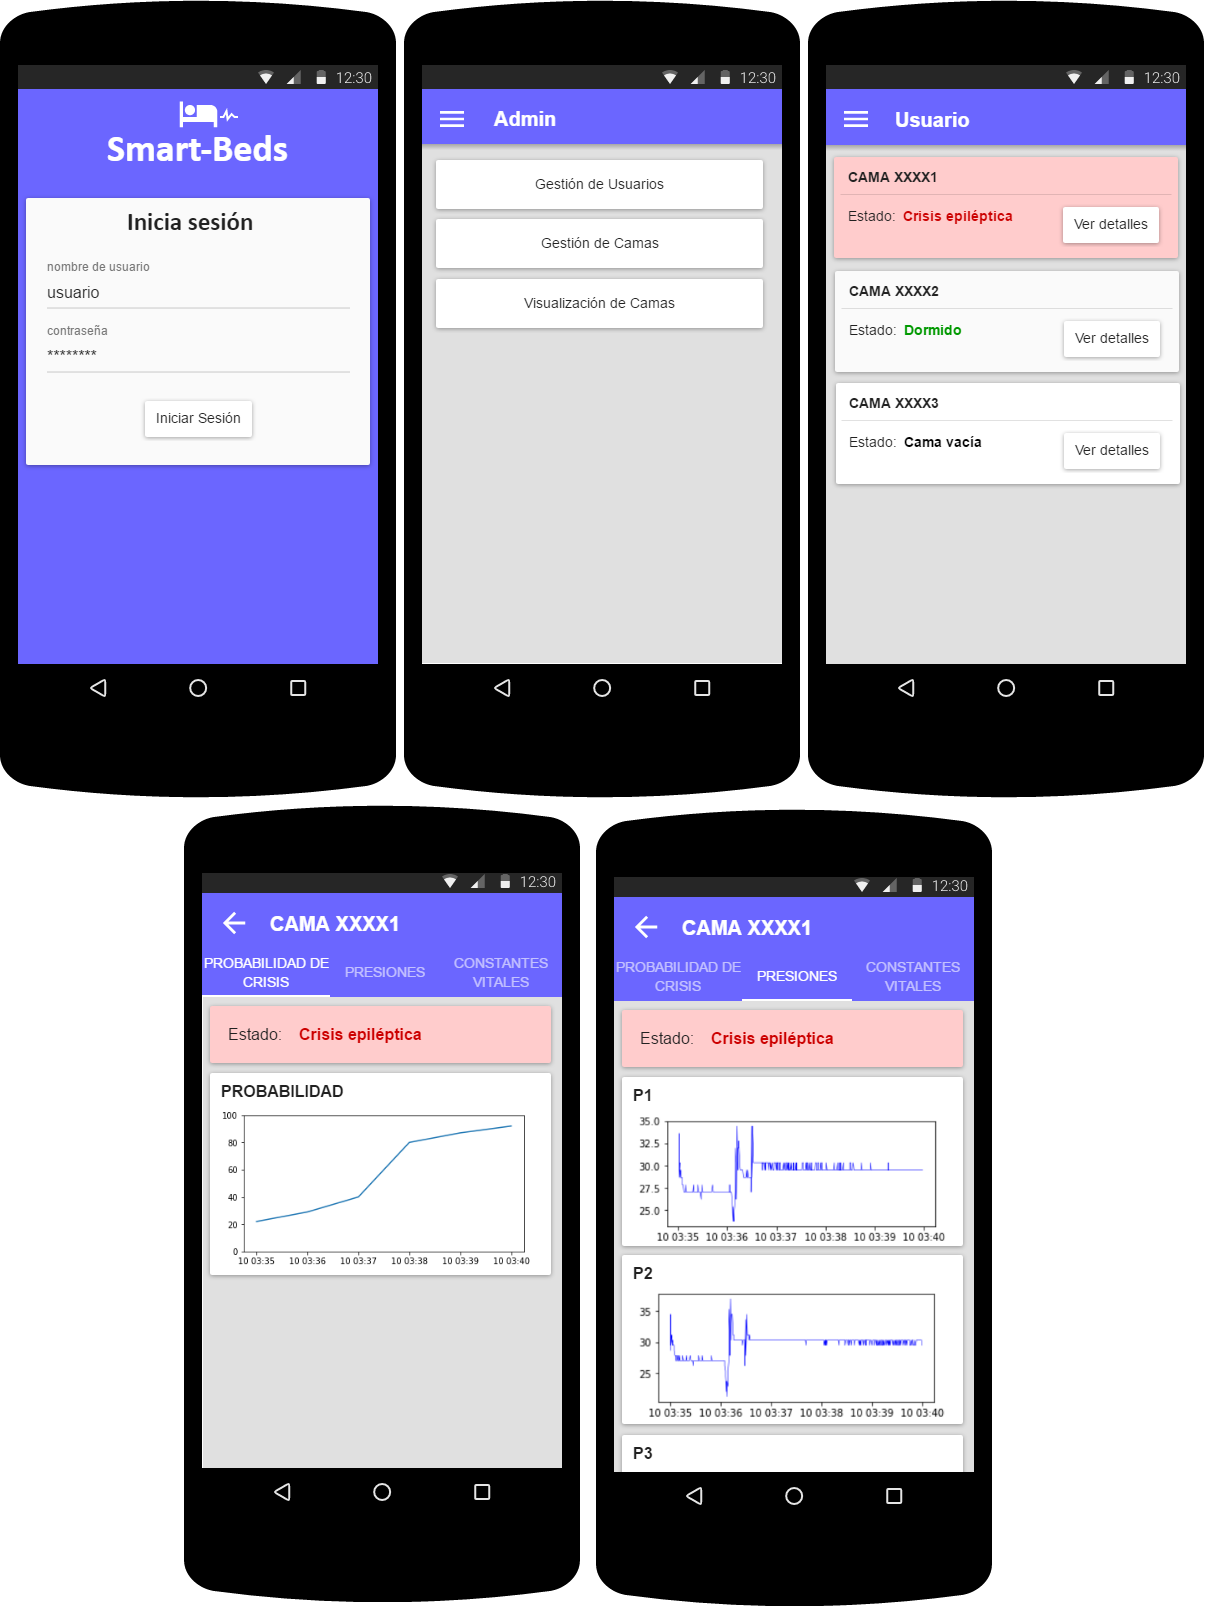
\includegraphics[width=0.75\textwidth]{../img/prototipos.png}
	\caption{Prototipos iniciales de las pantallas de: login, administración, visualización de camas y visualización de datos.}
	\label{fig:prototipos}
\end{figure}

Tal y como se recomienda en la guía de estilos y como se muestra en la figura~\ref{fig:paletacolores}, se escogieron dos colores principales para la interfaz: un color primario y un color secundario, más las consiguientes derivados de los mismos. 
\begin{itemize}
	\item El color primario y sus derivados se emplearon en las barras de herramientas, los botones y el menú de navegación. 
	\item El color secundario y su derivado se empleó para enfatizar elementos en los que el usuario debía realizar una acción, o elementos a los que debe prestar especial atención (como una cama en estado de crisis epiléptica). 
\end{itemize}

Además, para dar una sensación de claridad y limpieza, se decidieron mantener los fondos blancos, y el color del texto se estableció como claro (blanco) u oscuro (negro/gris) dependiendo del color del elemento donde se encontraba. De este modo se genera un contraste suficiente para que el texto resulte legible y claro. 

Los tamaños y separaciones entre textos y el resto de elementos se establecieron según las recomendaciones de la guía de estilos. 

\begin{figure}[H]
	\centering
	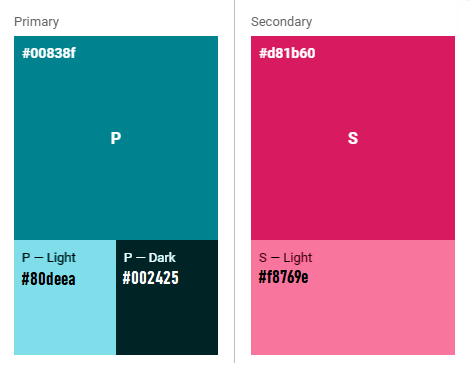
\includegraphics[width=0.8\textwidth]{../img/paletacolores.png}
	\caption{Paleta de colores.}
	\label{fig:paletacolores}
\end{figure}

Durante el proceso de desarrollo se tomaron varias decisiones de diseño cuyo resultado fueron las interfaces de usuario finales que se muestran en la figura~\ref{fig:interfaces}

\begin{figure}[H]
	\centering
	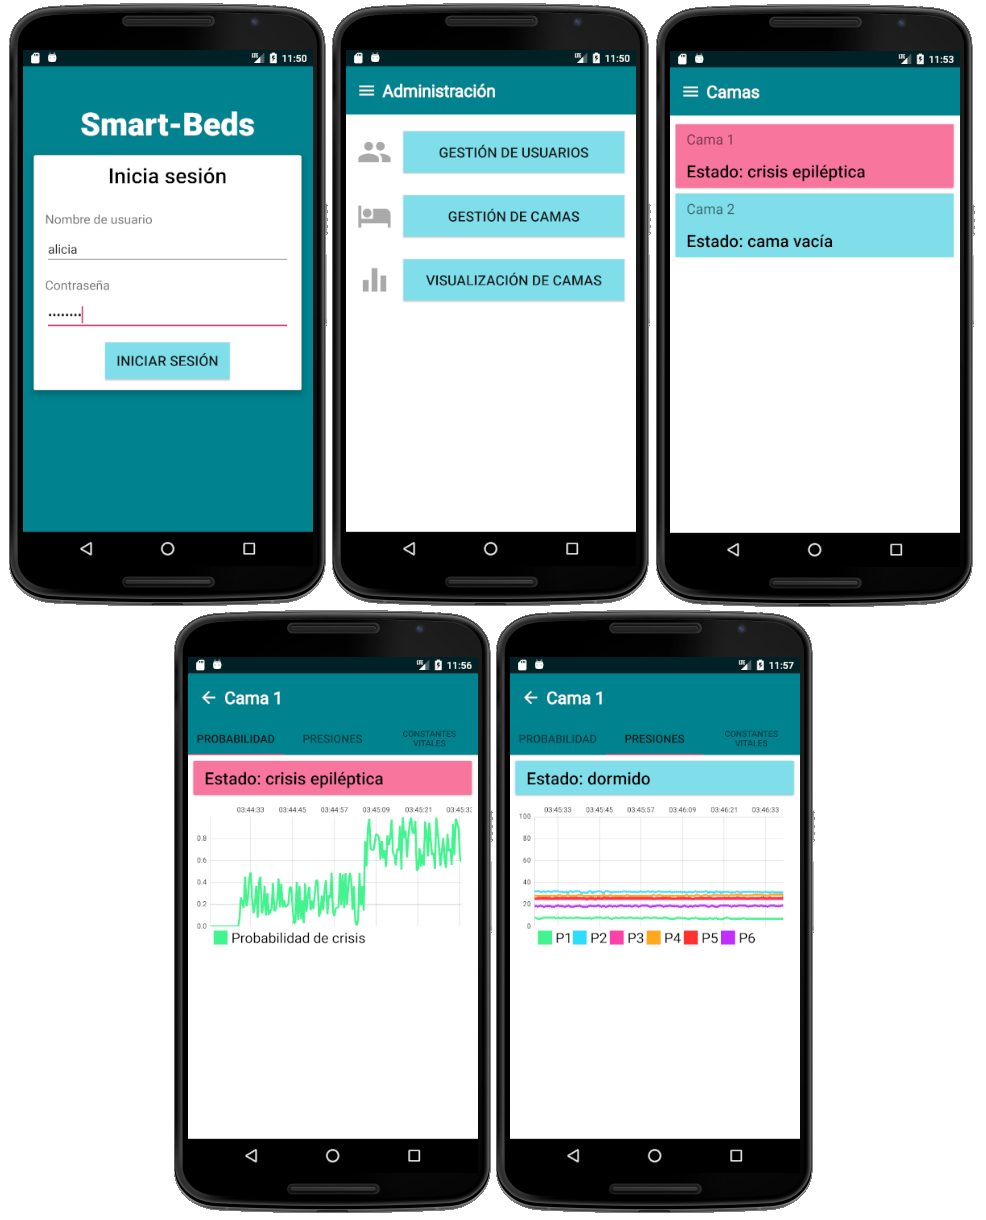
\includegraphics[width=0.75\textwidth]{../img/interfaces.png}
	\caption{Interfaces de usuario finales de las pantallas de: login, administración, visualización de camas y visualización de datos.}
	\label{fig:interfaces}
\end{figure}


\apendice{Documentación técnica de programación}

\section{Introducción}

En este apartado se van a exponer todos los conceptos necesarios para comprender la estructura de proyecto, instalar el software necesario para su integración, importarlo en un nuevo equipo, compilarlo, ejecutarlo y exportar la aplicación. 

Además, se exponen las herramientas que se han usado para generar las pruebas del software, se explica cómo usarlas para generar nuevas pruebas y cómo ejecutar las pruebas existentes. 

\section{Estructura de directorios}

En la figura~\ref{fig:directorios} se muestra la estructura de directorios del repositorio de GitHub en el que se encuentra alojado el proyecto: \url{https://github.com/aog0036/TFG-SmartBeds}. 

El contenido del repositorio se estructura principalmente en tres directorios: 
\begin{itemize}
	\item \textbf{/android:} Contiene el proyecto de Android Studio con los ficheros de código fuente, los de test, los de configuración y el fichro .apk generado. 
	\item \textbf{/doc:} Contiene la documentación general del proyecto, incluyendo la memoria, los anexos y el cuaderno de investigación, todos en formado .pdf y en formato .tex. También contiene otros recursos como las imágenes y los archivos con las referencias bibliográficas (extensión .bib). 
	\item \textbf{/jupyter notebooks:} Contiene los notebooks y los scripts de python con los experimentos generados durante la fase de investigación. 
\end{itemize}

Dentro del proyecto de Android Studio los directorios más importantes son los siguientes: 
\begin{itemize}
	\item \textbf{/app:} Contiene los directorios release, src y los que contienen los ficheros de pruebas unitarias y de interfaz. 
	\item \textbf{/app/release:} Contiene el fichero SmartBeds.apk para la instalación y distribución de la aplicación en un dispositivo Android. 
	\item \textbf{/app/src/main/java/.../smartbeds:} Contiene los paquetes con las clases Java que componen el código fuente de la aplicación. 
	\item \textbf{/app/src/main/res:} Contiene los directorios con los archivos .xml que definen los recursos gráficos de la aplicación (interfaces, colores, menús...). 
	\item \textbf{/app/src/main/AndroidManifest.xml:} Manifiesto que contiene información esencial sobre la aplicación y que permite al sistema ejecutarla. 
	\item \textbf{/app/src/androidTest/.../generalActivities:} Contiene las pruebas de interfaz gráfica generadas mediante la herramienta Espresso. 
	\item \textbf{/app/src/test/.../smartbeds:} Contiene las pruebas unitarias generadas mediante JUnit. 
	\item \textbf{/javadoc:} Contiene la documentación de las clases y métodos del código de la aplicación en formato html. 
	\item \textbf{archivos de configuración de gradle:} Son una serie de directorios y ficheros generados automáticamente por Android Studio y que permiten construir la aplicación con la configuración y las dependencias necesarias. 
\end{itemize}

\begin{figure}
	\centering
	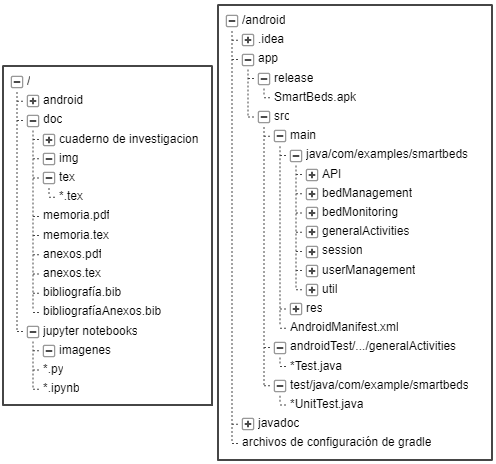
\includegraphics[width=1\textwidth]{../img/directorios.png}
	\caption{Estructura de directorios del repositorio.}
	\label{fig:directorios}
\end{figure}

\section{Manual del programador}

\subsection{Experimentos} 

En el repositorio no se incluye el directorio /data con los ficheros .csv ya que estos datos son propiedad de la empresa proveedora de los datos, por lo que no es posible ejecutar los experimentos, pero sí se pueden visualizar los procesos que se han seguido en cada uno de ellos, los distintos métodos que se han empleado y los resultados conseguidos. Para ello es necesario tener instalada la herramienta Jupyter Notebook. 

En caso de heredar este proyecto y contar con el directorio /data que contiene los datos proporcionados por el proveedor, se recomienda instalar Anaconda, ya que además de incluir Jupyter Notebook, instala por defecto muchas de las bibliotecas que se emplean en los experimentos. Todos los experimentos se han escrito en código de \textbf{Python 3}. 

\subsection{Aplicación Android}

Para trabajar con el proyecto de Android Studio es necesario tener instalado \textbf{Java JDK 8} y \textbf{Android Studio}. En este caso se ha usado una versión de Android Studio 3.3.2. El resto de dependencias se encuentran indicadas en los ficheros de configuración de gradle, y se añaden automáticamente al construir la aplicación. Concretamente las dependencias de la aplicación se encuentran en el fichero \textbf{/android/app/build.gradle}, y será aquí donde se deberán añadir las dependencias nuevas si son necesarias. En este archivo también se indica la versión mínima de la API de Android que se soporta, en este caso la 23, que corresponde con la versión 6 de Android (\textit{Marshmallow}). Esto supone que la aplicación funcionará en dispositivos con una versión 6 de Android o superior. 

Además, el funcionamiento de esta aplicación depende de los servicios ofrecidos por la API implementada por mi compañero José Luis Garrido Labrador. Los requisitos e instalación de la API del servidor remoto se encuentran documentados en los anexos de su trabajo: \url{https://github.com/jlgarridol/TFG-SmartBeds}.

\section{Compilación, instalación y ejecución del proyecto}

En este apartado se indica cómo importar el proyecto de Android Studio, cómo ejecutar la aplicación y cómo exportar el archivo .apk para la distribución en instalación de la aplicación en un dispositivo Android. 

\subsection{Importar el proyecto}

Una vez instalados Java JDK 8 y Android Studio, para importar el proyecto se deben seguir los siguientes pasos: 

\begin{enumerate}
	\item Acceder al repositorio: \url{https://github.com/aog0036/TFG-SmartBeds}. 
	\item Descargar el contenido del repositorio desde \textbf{Clone or download >~Download ZIP}. 
	\begin{figure}[H]
		\centering
		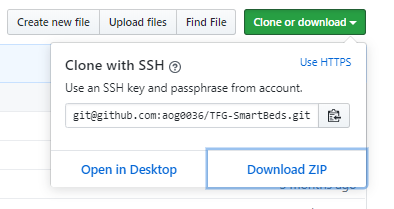
\includegraphics[width=0.5\textwidth]{../img/download.png}
		\caption{Descarga del contenido del repositorio.}
		\label{fig:download}
	\end{figure}
	\item Descomprimir el fichero .zip en la ruta en la que se desee alojar el proyecto. 
	\item Abrir Android Studio. 
	\item En el menú de opciones de Android Studio ir a \textbf{File >~Open} y seleccionar el directorio \textbf{/android}. 
	\begin{figure}[H]
		\centering
		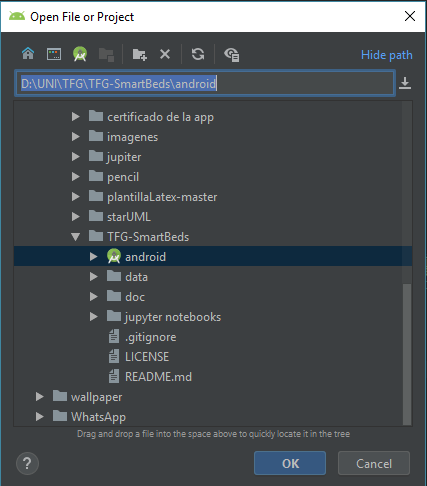
\includegraphics[width=0.5\textwidth]{../img/open.png}
		\caption{Importar proyecto de Android Studio.}
		\label{fig:open}
	\end{figure}
\end{enumerate}

\subsection{Ejecutar la aplicación}

Existen dos formas de ejecutar la aplicación en Android Studio: conectando tu dispositivo Android mediante USB o usando un emulador. Para que tu equipo reconozca tu dispositivo Android al conectarlo es necesario que tengas instalados sus \textit{drivers}, por lo demás, es la opción más rápida y cómoda. Por otro lado, si no cuentas con un dispositivo que tenga una versión de Android compatible con la aplicación, puedes crear un nuevo emulador de la siguiente forma: 

\begin{enumerate}
	\item En el menú de opciones ir a \textbf{Run >~Run 'app'}. 
	\item En la ventana emergente que se muestra seleccionar la opción \textbf{Create New Virtual Device}. 
	\item Aquí podrás escoger el modelo del dispositivo que quieras emular y la versión de Android a instalar. 
\end{enumerate}

Para ejecutar la aplicación, tanto en un dispositivo conectado al equipo como en el emulador, se siguen los siguientes pasos: 

\begin{enumerate}
	\item En el menú de opciones ir a \textbf{Run >~Run 'app'}.
	\item En la ventana emergente seleccionar el dispositivo que quieres usar y pulsar \textbf{OK}. 
\end{enumerate}

\subsection{Exportar apk}

Para exportar el archivo .apk que permite distribuir e instalar la aplicación en un dispositivo Android se siguen los siguientes pasos: 

\begin{enumerate}
	\item En el menú de opciones ir a \textbf{Build >~Build Bundle(s) / APK(s) >~Build APK(s)}. 
	\item El archivo apk generado se encontrará en el directorio \\ \textbf{/android/app/build/outputs/apk/debug}.
\end{enumerate}

Si se desea generar un apk para subirlo a la plataforma Google Play se debe escoger la opción \textbf{Build >~Generate Signed Build / APK...} que crea una apk firmada, asociada a un certificado que es necesario para distribuir la aplicación en Google Play. 

\section{Pruebas del sistema}

Además de las pruebas manuales, se han realizado dos tipos de pruebas del sistema: pruebas unitarias y pruebas de sistema, más concretamente de interfaz de usuario. 

\subsection{Pruebas unitarias} 

Para realizar las pruebas unitarias sobre las clases que no están directamente asociadas con una interfaz de usuario se ha empleado la biblioteca de pruebas unitaria sobre Java \textbf{JUnit}. Las pruebas unitarias comprueban el buen comportamiento de un solo módulo o clase de forma aislada.

Estas pruebas se encuentran en el directorio \\ \textbf{/android/app/src/test/java/com/example/smartbeds}. 

\subsection{Pruebas de interfaz}

Además de las pruebas unitarias, se han realizado una serie de pruebas sobre la interfaz de usuario mediante la herramienta \textbf{Espresso}. Esta herramienta permite grabar las acciones del usuario sobre los elementos de la interfaz de usuario, hacer comprobaciones del contenido tras cada acción y volver a ejecutar la grabación. Este tipo de pruebas resultan más útiles para una aplicación pequeña como esta. 

Para ejecutar las pruebas unitarias debemos seleccionar el directorio que las contiene en el menú de navegación del proyecto y pulsar \textbf{Run 'Tests in 'nombre del directorio''}. 

Además, la herramienta Espresso se encuentra completamente integrada en Android Studio, permitiendo generar una nueva prueba de la siguiente forma:

\begin{enumerate}
	\item En el menú de opciones de Android Studio ir a \textbf{Run >~Record Espresso Test}. 
	\item Escoger el dispositivo (real o emulado) sobre el que se desea grabar la prueba y pulsar \textbf{OK}. 
	\item Se abrirá una ventana emergente en la que se irán registrando las acciones. 
	\item Tras cada acción, pulsando en la opción \textbf{Add Assertion} de la ventana emergente se pueden añadir comprobaciones sobre el contenido de la interfaz (por ejemplo, comprobar que cierto elemento está presente o que cierto \textit{TextView} contiene un texto determinado). 
	\item Una vez realizada la grabación al pulsar \textbf{OK} se generará el código correspondiente de la prueba con el nombre que se le indique. 
\end{enumerate} 

Para ejecutar la prueba generada debemos seleccionarla en el menú de navegación del proyecto con click derecho y seleccionar \textbf{Run 'nombre del test'}. También podemos ejecutar todas las pruebas seleccionando con click derecho el directorio que las contiene y pulsando \textbf{Run 'Tests in 'nombre del directorio''}. 

Estas pruebas se encuentran en el directorio \\ \textbf{/android/app/src/androidTest/java/com/example/smartbeds/\\generalActivities}.


\apendice{Documentación de usuario}

\section{Introducción}

En esta sección se enumeran los requisitos que debe cumplir el usuario para poder usar la aplicación, se explica el proceso de instalación y se ofrece un manual de usuario completo para aprender a usarla. 

\section{Requisitos de usuarios}

Para poder instalar y usar la aplicación el dispositivo del usuario debe complir los siguientes requisitos: 

\begin{itemize}
	\item Contar con una versión de Android 6 (\textit{Marshmallow}) o superior, la cual corresponde con la API 23 de Android. 
	\item Permitir la instalación de aplicaciones de orígenes desconocidos~\cite{origenesdesconocidos}. Para ello: 
	\begin{enumerate}
		\item Ir a los ajustes del dispositivo. 
		\item A la opción de \textbf{Seguridad} o \textbf{Privacidad} según la versión. 
		\item Activar la opción \textbf{Orígenes desconocidos}. 
	\end{enumerate}
	\item Contar con conexión a internet. 
\end{itemize}

Además, para poder entrar en la aplicación deberá tener un usuario y una contraseña asignados. 

\section{Instalación}

La instalación de una aplicación Android es muy sencilla. Solo es necesario pasar el archivo \textbf{SmartBeds.apk} al sistema de ficheros del dispositivo Android y seleccionarlo. En caso de tener activada la opción de permitir la instalación de aplicaciones de orígenes desconocidos y contar con el suficiente espacio de almacenamiento la aplicación se instalará automáticamente. 

Se recuerda que el archivo .apk se encuentra en el repositorio del proyecto\footnote{\url{https://github.com/aog0036/TFG-SmartBeds}}, en la ruta \textbf{/android/app/release}.

\section{Manual del usuario}

En esta sección se ofrece un manual para el uso sobre todas las funcionalidades de la aplicación. 

\subsection{Iniciar sesión}

Al ejecutar la aplicación desde el dispositivo Android la primera pantalla que se muestra es la de <<\textbf{Iniciar Sesión}>>. En esta pantalla se nos pide un nombre de usuario y una contraseña para acceder al sistema. Se debe: 

\begin{enumerate}
	\item Introducir el nombre de usuario. 
	\item Introducir la contraseña. 
	\item Pulsar el botón <<Iniciar sesión>>. 
\end{enumerate}

En caso de haber introducido valores correctos se accederá a la siguiente pantalla, en caso contrario un cuadro de diálogo nos indicará que el usuario o la contraseña introducidos no son correctos. 

Si el usuario introducido tiene un rol de administrador la siguiente pantalla será el <<\textbf{Menú de administración}>>. Si tiene un rol de usuario la siguiente pantalla será la de <<\textbf{Visualización de camas}>>. 

\begin{figure}[H]
	\centering
	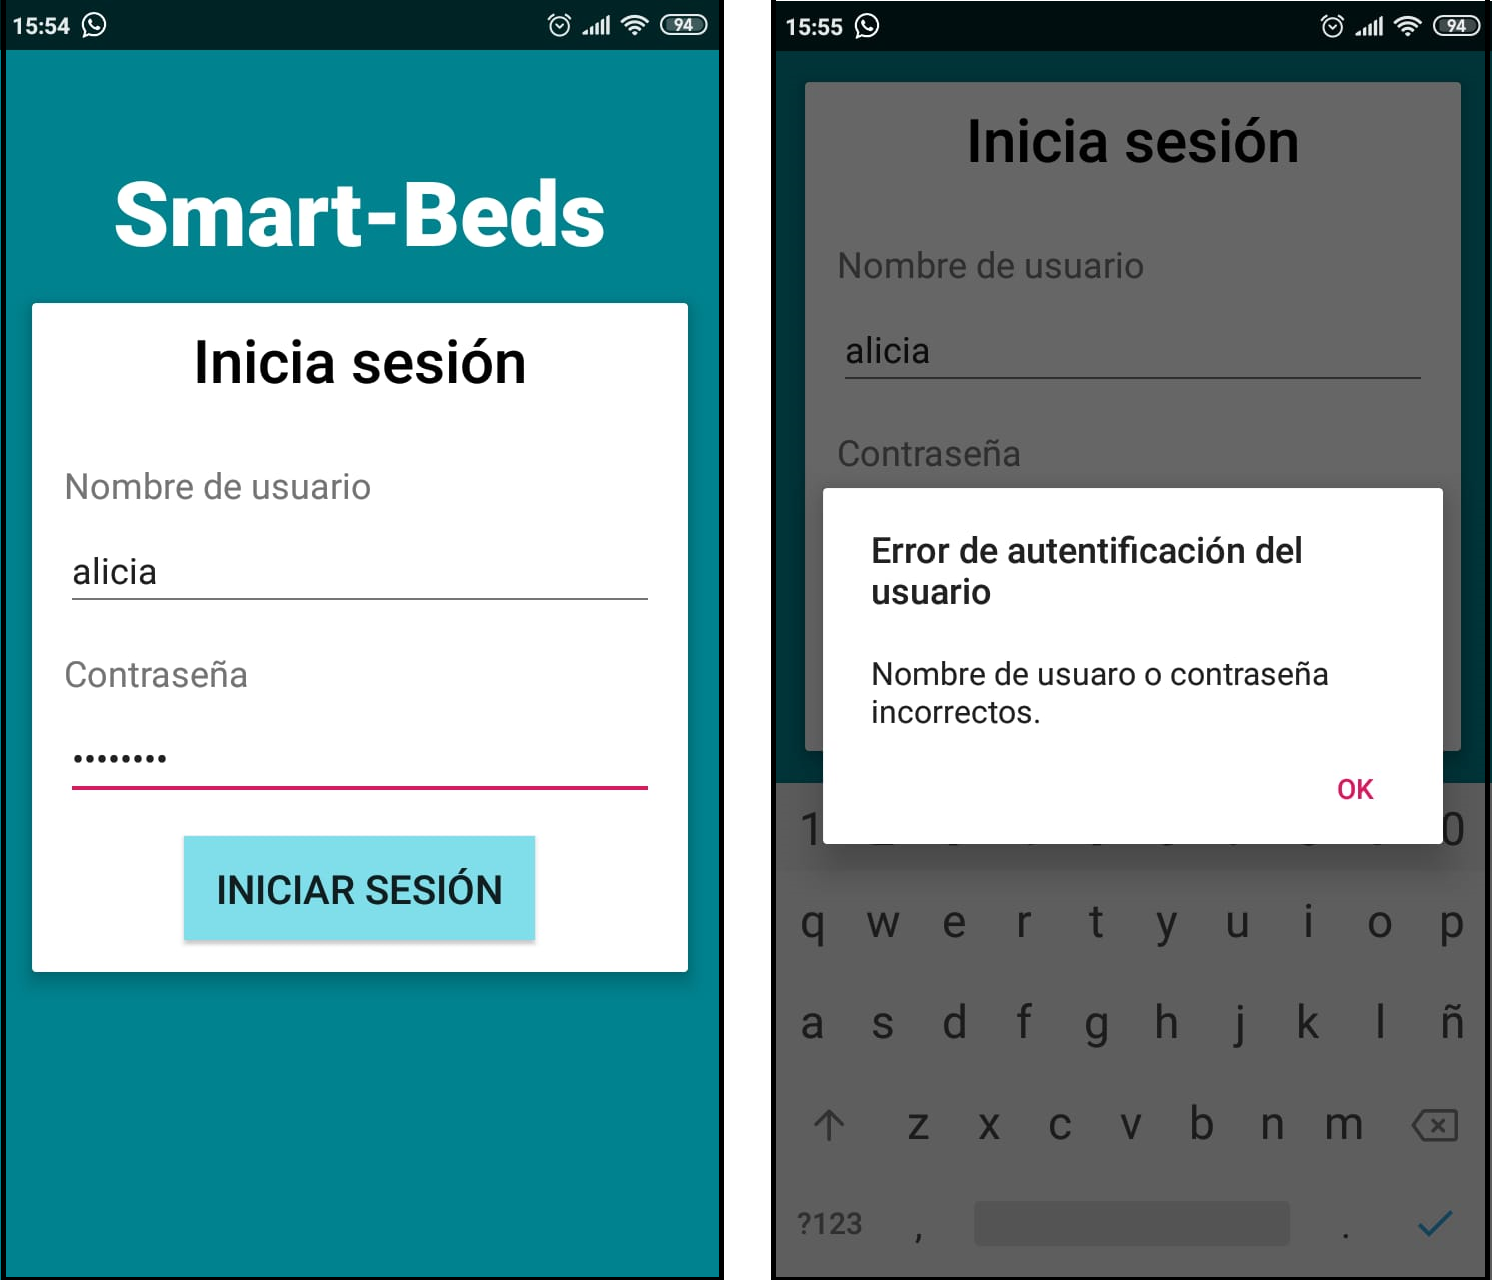
\includegraphics[width=0.7\textwidth]{../img/iniciasesion.png}
	\caption{Iniciar sesión.}
	\label{fig:iniciasesion}
\end{figure}

\subsection{Menú de administración}

Este menú solo está disponible si el usuario tiene un rol de administrador. En él puedes escoger a qué función de la aplicación deseas acceder: <<\textbf{Gestión de usuarios}>>, <<\textbf{Gestión de camas}>> o <<\textbf{Visualización de camas}>>. 

\begin{figure}[H]
	\centering
	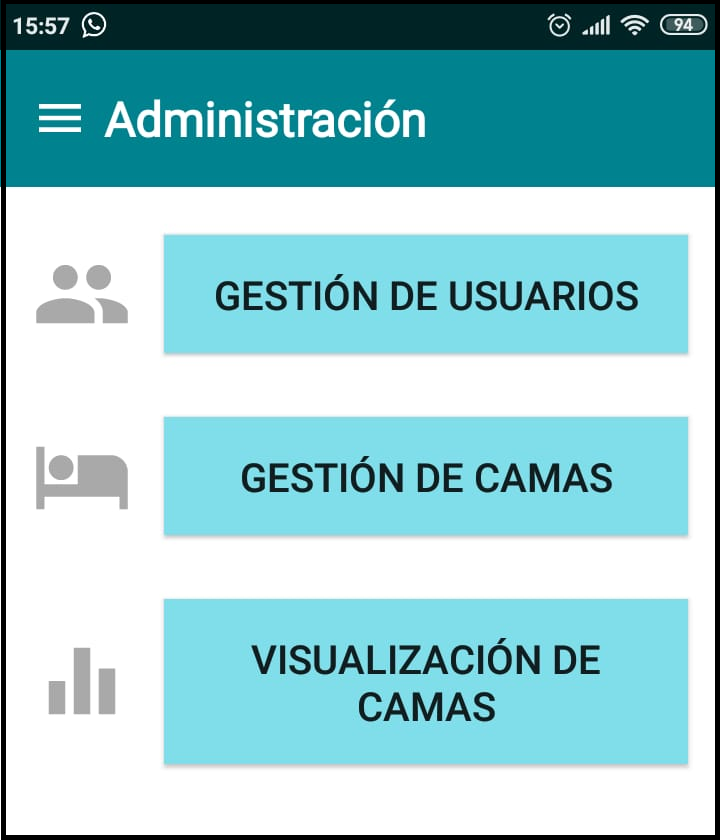
\includegraphics[width=0.4\textwidth]{../img/menudeadministracion.png}
	\caption{Menú de administración.}
	\label{fig:menudeadministracion}
\end{figure}

\subsection{Gesión de usuarios}

Esta pantalla solo está disponible si el usuario tiene un rol de administrador. En esta pantalla se muestra una lista de todos los usuarios registrados en el sistema. Al mantener pulsado uno de ellos queda seleccionado y se muestran las opciones disponibles: <<\textbf{Cambiar contraseña}>> y <<\textbf{Eliminar}>>.

\begin{itemize}
	\item Si escogemos <<\textbf{Cambiar contraseña}>> se muestra una pantalla donde debemos introducir dos veces la nueva contraseña y pulsar el botón <<Cambiar contraseña>>.
	\item Si escogemos <<\textbf{Eliminar}>> aparece un cuadro de diálogo preguntando al usuario si desea eliminar de forma permanente al usuario seleccionado. 
	\item Para \textbf{añadir un nuevo usuario} al sistema debemos pulsar en el símbolo <<+>> en la esquina inferior derecha de la pantalla, la cual nos llevará a una pantalla donde deberemos introducir el nombre de usuario y la contraseña del nuevo usuario, y pulsar el botón <<Añadir usuario>>. 
\end{itemize}  

\begin{figure}[H]
	\centering
	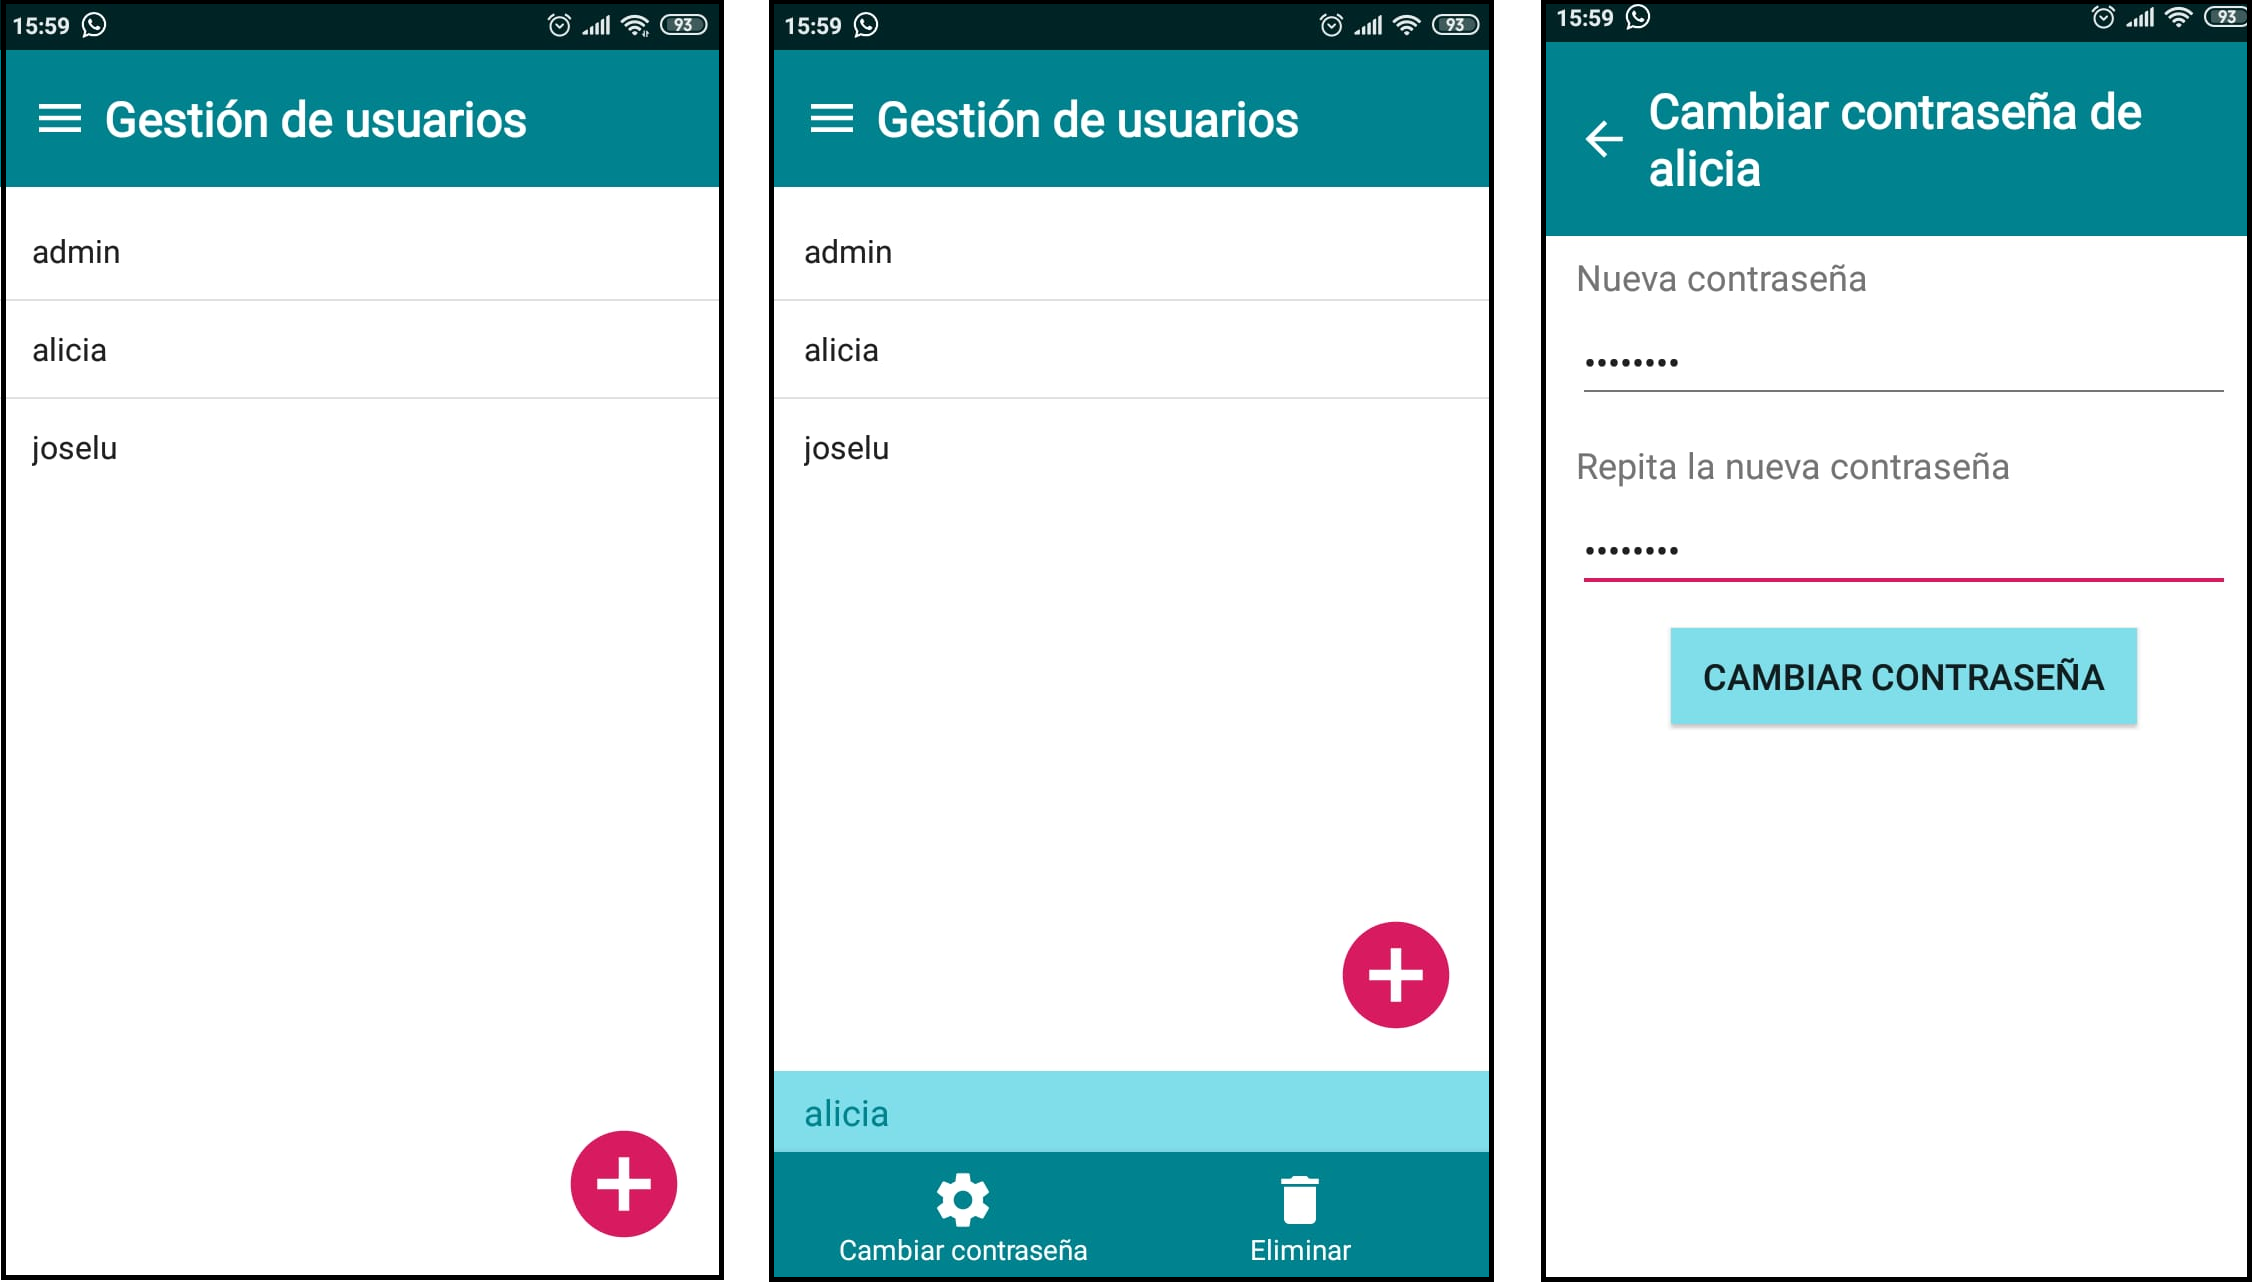
\includegraphics[width=1\textwidth]{../img/gestiondeusuarios.png}
	\caption{Gestión de usuarios, cambiar contraseña.}
	\label{fig:gestiondeusuarios}
\end{figure}

\begin{figure}[H]
	\centering
	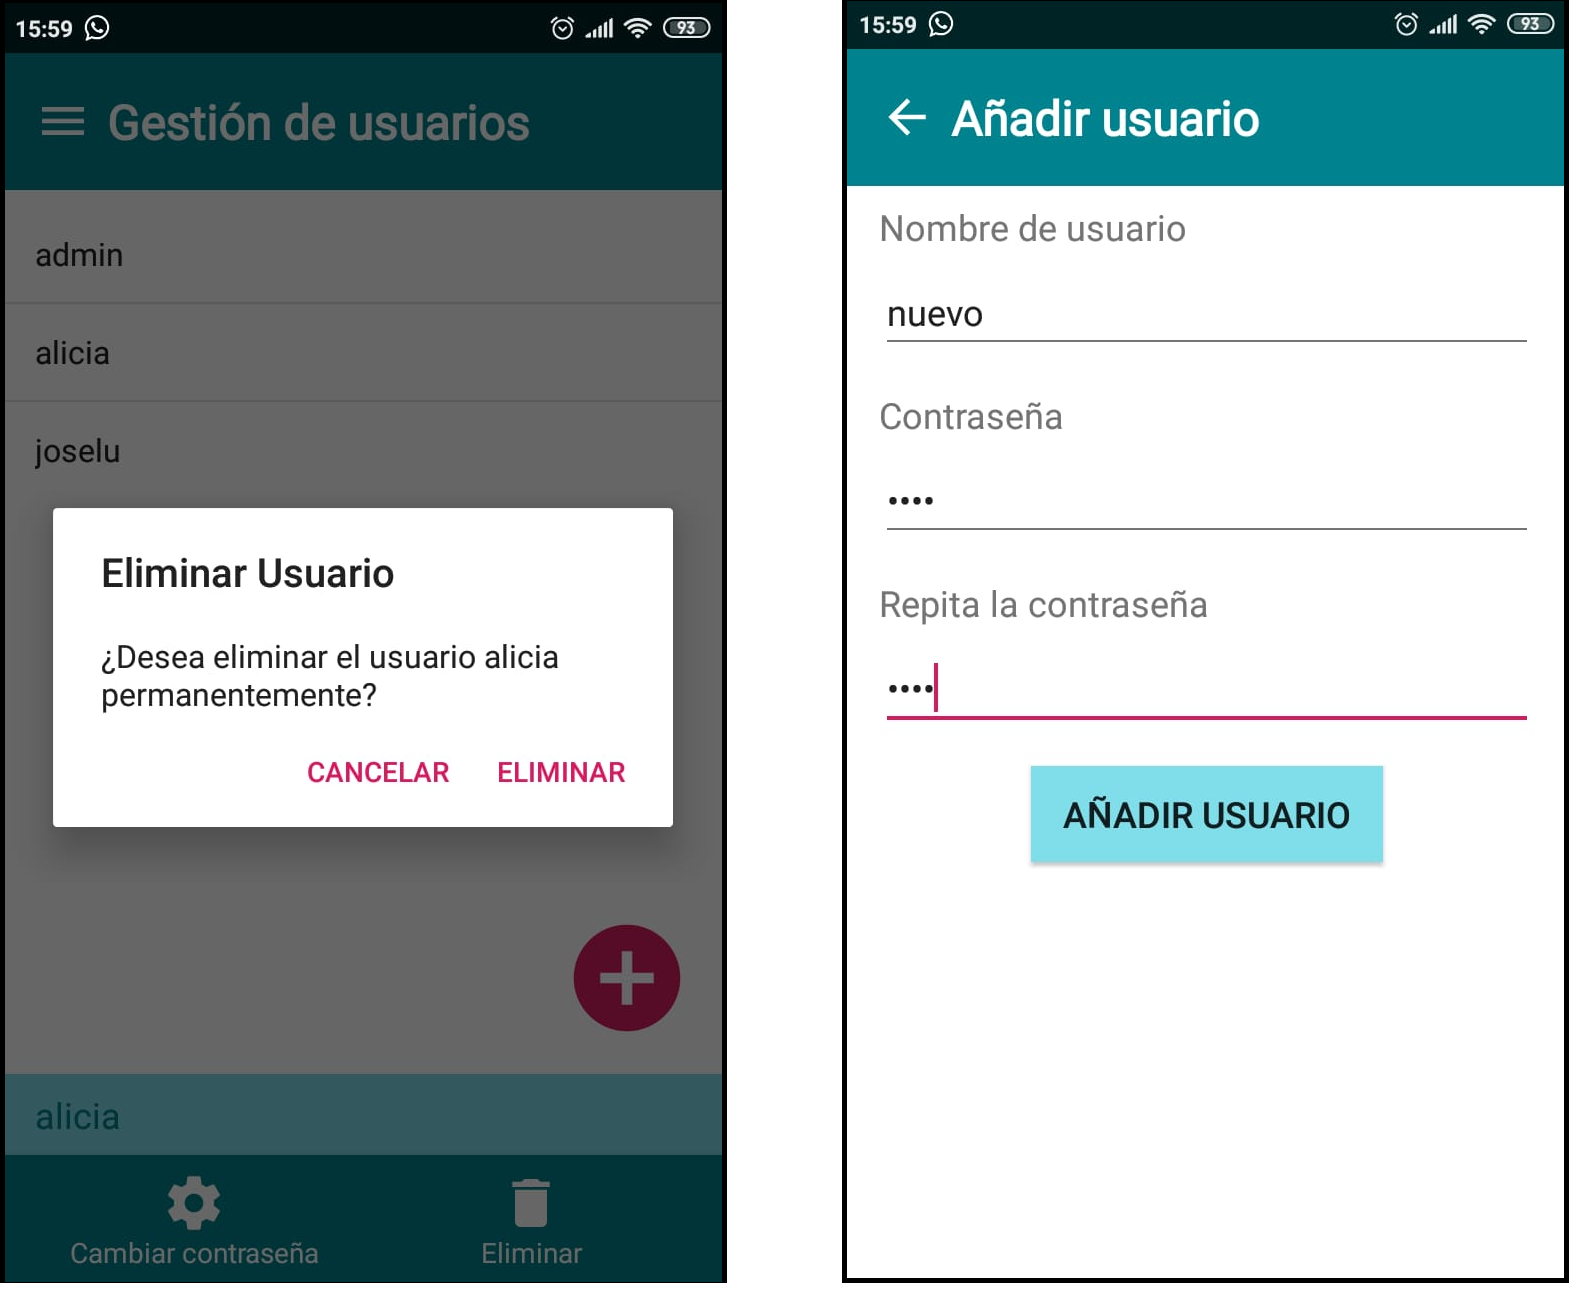
\includegraphics[width=0.7\textwidth]{../img/eliminaranadir.png}
	\caption{Gestión de usuarios, eliminar y añadir usuarios.}
	\label{fig:eliminaranadir}
\end{figure}

\subsection{Gestión de camas}

Esta pantalla solo está disponible si el usuario tiene un rol de administrador. En esta pantalla se muestra una lista de todas las camas registradas en el sistema. Al mantener pulsada una de ellas queda seleccionada y se muestran las opciones disponibles: <<\textbf{Modificar}>>, <<\textbf{Eliminar}>> y <<\textbf{Asignar usuarios}>>.  

De estas tres funciones, en esta versión de la aplicación solo está disponible la de \textbf{Asignar usuarios}, al seleccionar el resto solo se muestra un cuadro de diálogo informativo. Seleccionar la opción <<Asignar usuarios>> lleva a una pantalla donde se muestra una lista de todos los usuarios del sistema. En esta lista se pueden marcar aquellos que se desea que puedan ver la cama seleccionada y desmarcar los que no.

Según la figura~\ref{fig:gestiondecamas} el usuario <<joselu>> tendría acceso a los datos de la <<Cama 1>> pero el usuario <<alicia>> no. 

\begin{figure}[H]
	\centering
	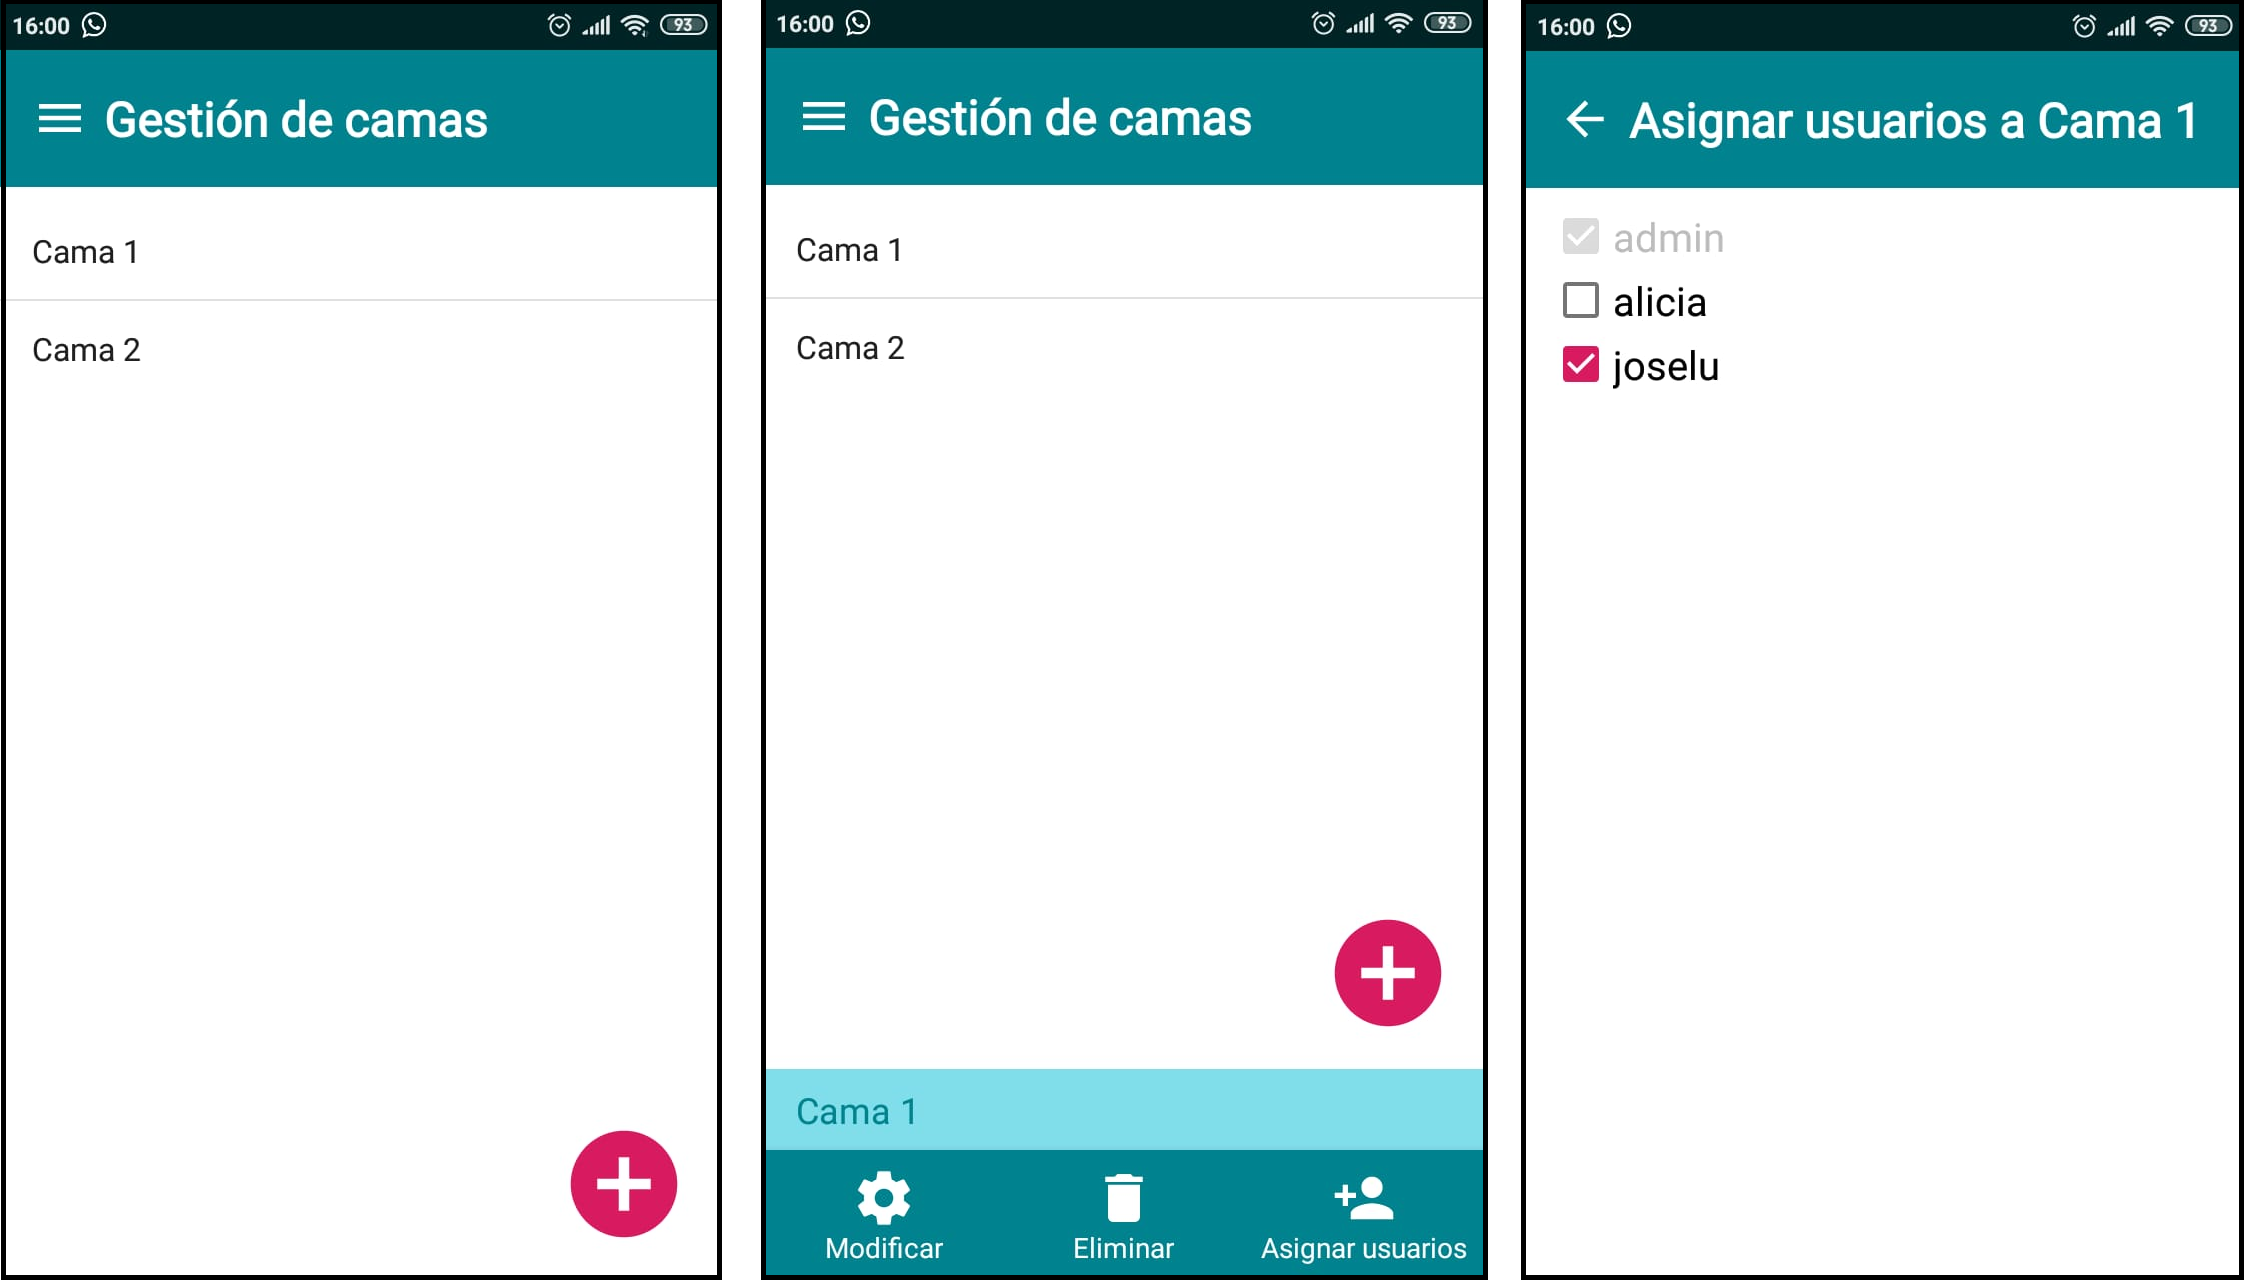
\includegraphics[width=0.9\textwidth]{../img/gestiondecamas.png}
	\caption{Gestión de camas, asignar usuarios.}
	\label{fig:gestiondecamas}
\end{figure}

\subsection{Visualización de camas}

Esta pantalla está disponible para usuarios con un rol de administrador y con un rol de usuario normal. Los administradores tendrán visibles todas las camas del sistema, los usuarios normales solo aquellas que el administrador les haya asignado. 

La pantalla muestra una lista de camas junto con el estado del paciente asociado en tiempo real (<<dormido>>, <<crisis epiléptica>>, <<cama vacía>> o <<datos insuficientes>>). Al pulsar una de las camas se accede a la pantalla de <<\textbf{Visualización de los datos de una cama en tiempo real}>>. 

\begin{figure}[H]
	\centering
	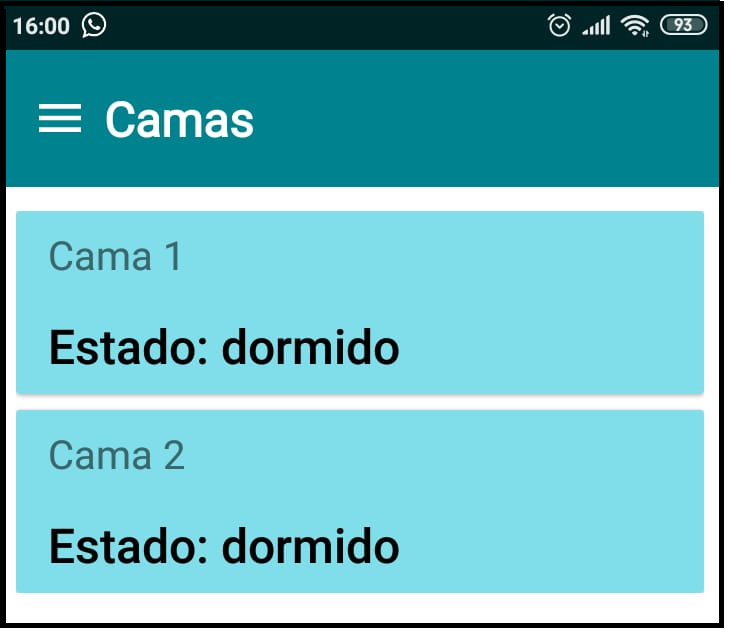
\includegraphics[width=0.4\textwidth]{../img/visualizaciondecamas.png}
	\caption{Visualización de camas.}
	\label{fig:visualizaciondecamas}
\end{figure}

\subsection{Visualización de los datos de una cama en tiempo real}

Esta pantalla está disponible para usuarios con un rol de administrador y con un rol de usuario normal. Un usuario normal solo podrá acceder a la pantalla asociada a una cama concreta si tiene permisos para visualizar esa cama. 

Como se aprecia en la figura~\ref{fig:datoscama}, esta pantalla se divide en tres pestañas que contienen distintas gráficas cuyos datos se actualizan en tiempo real: 

\begin{itemize}
	\item La primera contiene una gráfica con la \textbf{probabilidad} de que el paciente esté sufriendo una crisis epiléptica. 
	\item La segunda contiene una gráfica que muestra \textbf{una línea de datos por cada sensor de presión} instalado en el interior del colchón. 
	\item La tercera contiene cinco gráficas relativas a las \textbf{constantes vitales} del paciente: 
	\begin{itemize}
		\item Frecuencia cardíaca (pulsaciones/minuto)
		\item Frecuencia respiratoria (respiraciones/minuto)
		\item Volumen sistólico (mililitros)
		\item Variabilidad de la frecuencia cardíaca (milisegundos)
		\item Tiempo entre pulsaciones (milisegundos)
	\end{itemize}
\end{itemize}

\begin{figure}[H]
	\centering
	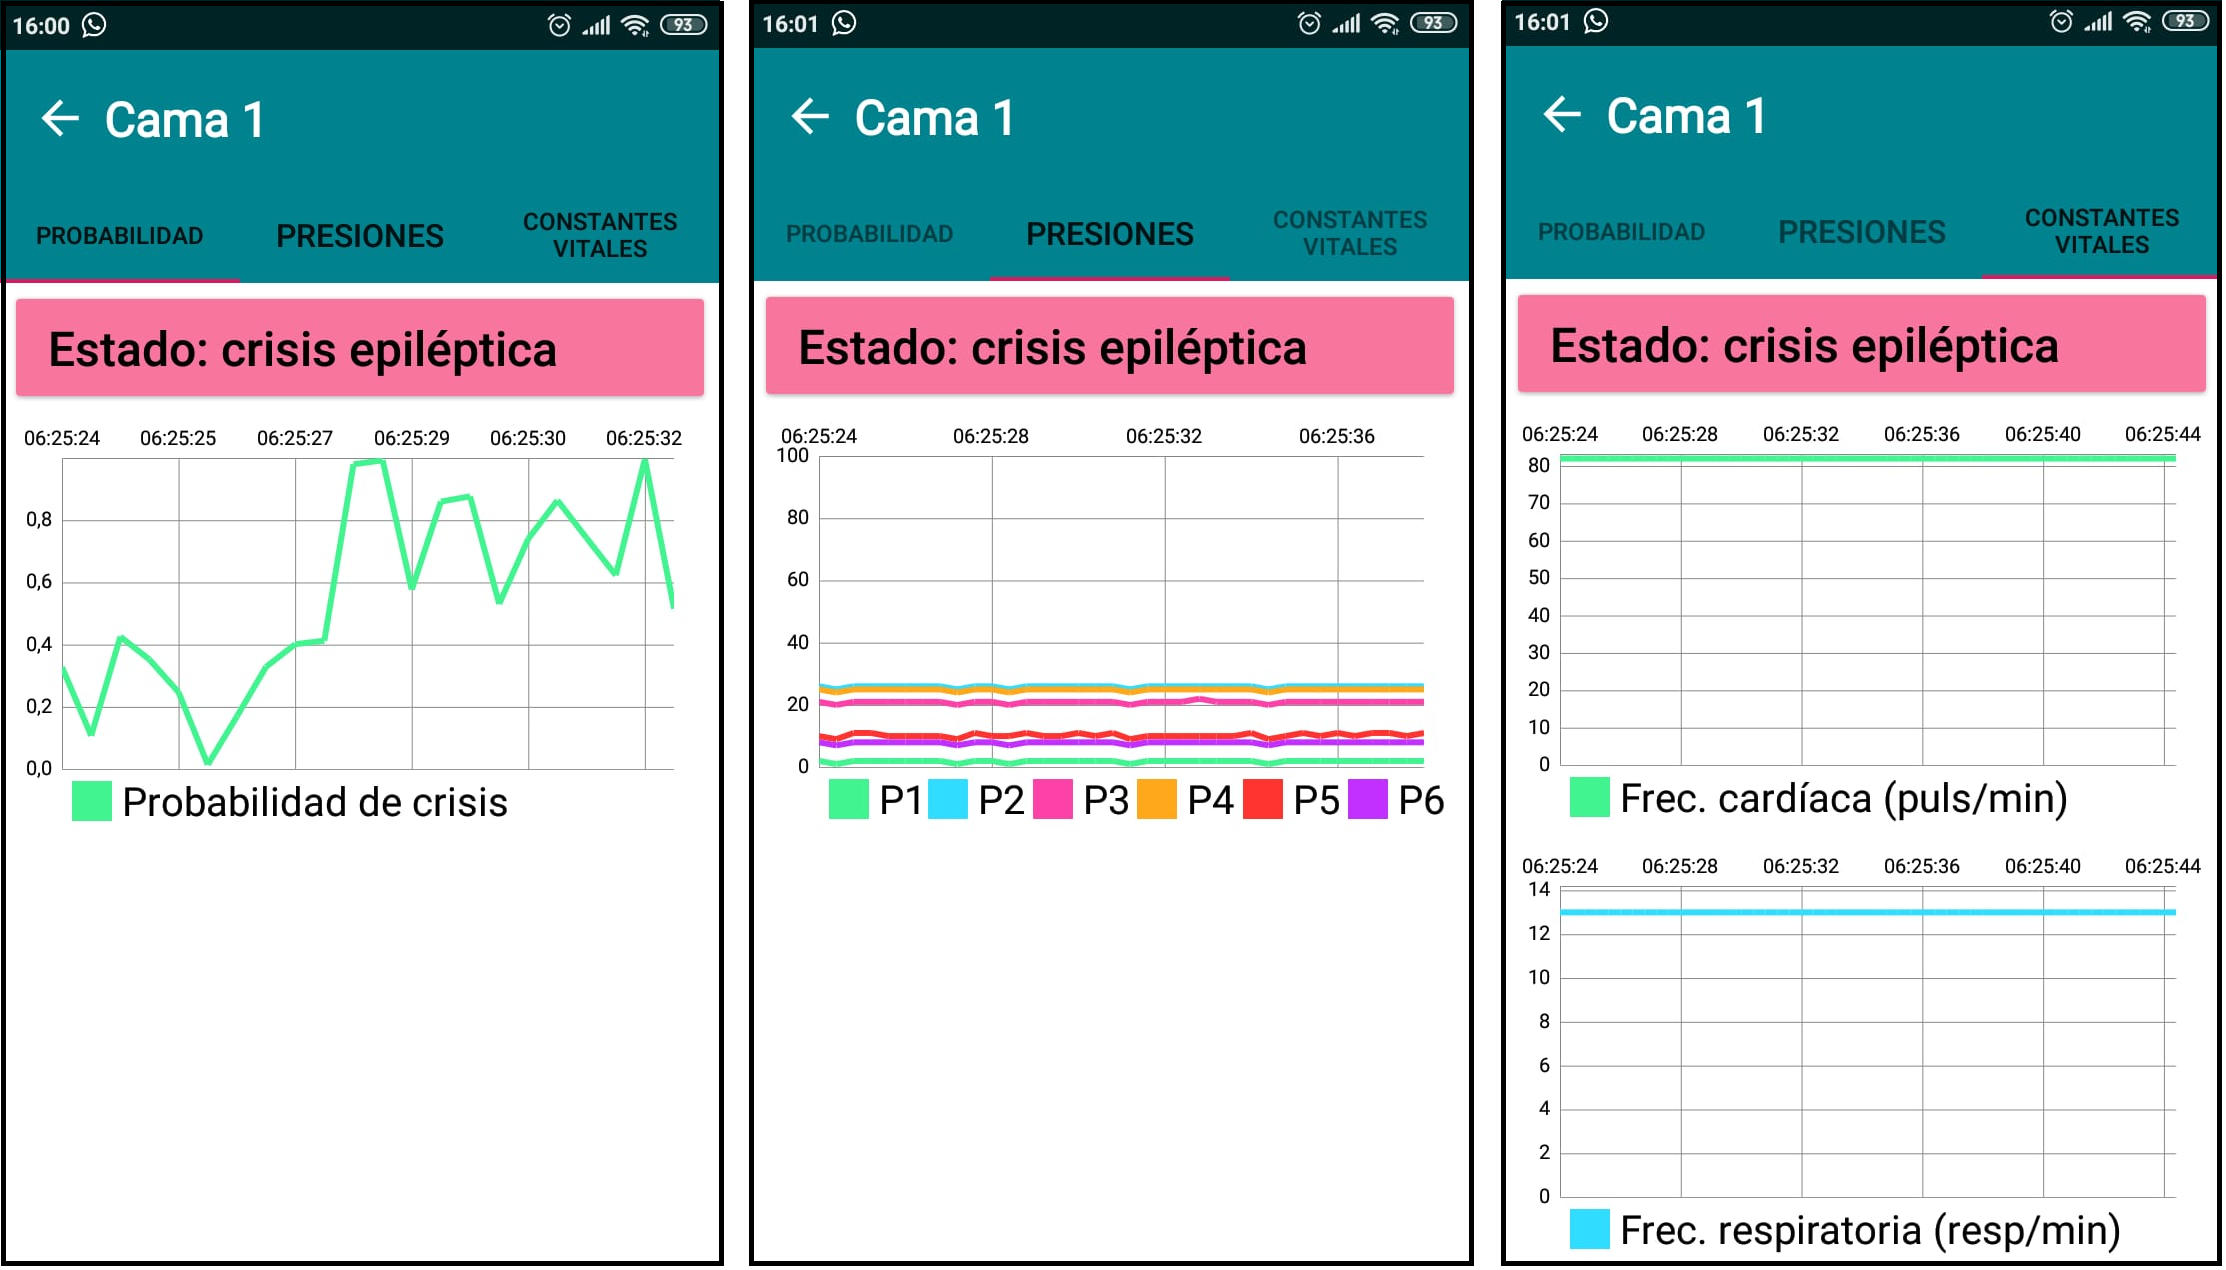
\includegraphics[width=0.9\textwidth]{../img/datoscama.png}
	\caption{Visualización de los datos de una cama en tiempo real.}
	\label{fig:datoscama}
\end{figure}

\subsection{Menú de navegación}

En las pantallas en las que se puede ver un icono de menú en la esquina superior izquierda es posible desplegar un menú de navegación pulsando el icono o deslizando el dedo por la pantalla de izquierda a derecha. Como se aprecia en la figura~\ref{fig:menunavegacion}, este menú contiene opciones distintas si se trata de un usuario con rol de administrador o un usuario normal. 

Para un usuario administrador incluye las mismas opciones que para un usuario normal y adicionalmente, las opciones del menú de administración. De esta forma se proporciona al administrador otra forma de navegar por la aplicación. Además de estas opciones se muestran tres más: <<\textbf{Modificar contraseña}>>, <<\textbf{Acerca de}>> y <<\textbf{Cerrar sesión}>>. La opción <<Cerrar sesión>> devuelve al usuario a la página inicial, las otras dos opciones llevan a sus respectivas pantallas.  

\begin{figure}[H]
	\centering
	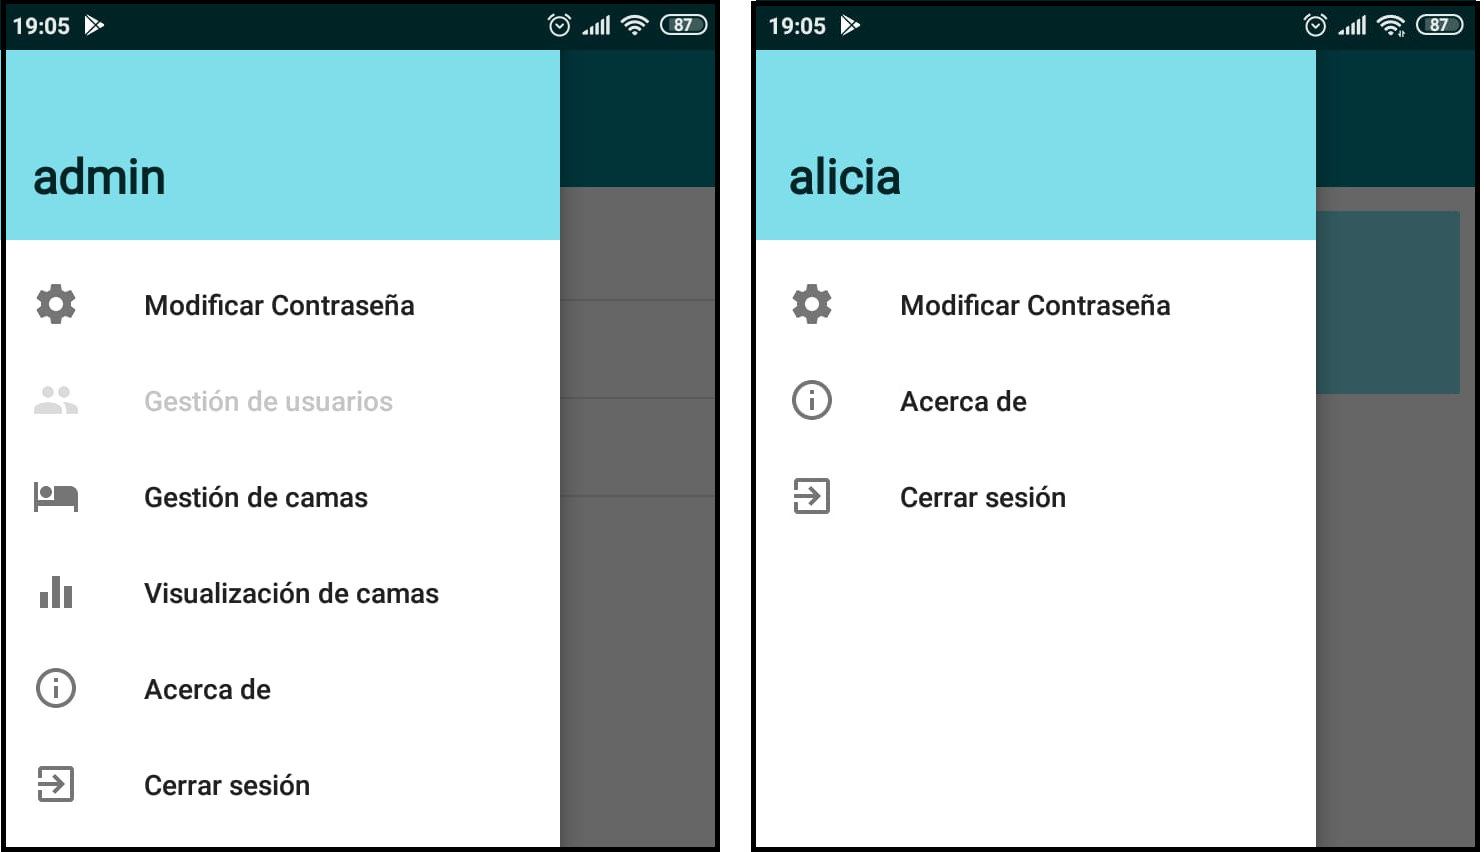
\includegraphics[width=0.7\textwidth]{../img/menunavegacion.png}
	\caption{Menú de navegación para un administrador y para un usuario normal.}
	\label{fig:menunavegacion}
\end{figure} 

\subsection{Modificar contraseña}

Hemos visto que el administrador puede cambiar la contraseña de cualquier usuario del sistema, pero mediante la opción <<Modificar contraseña>> del menú de navegación se permite cambiar la contraseña del usuario que se encuentra identificado en el sistema. En esta pantalla se debe introducir una vez la antigua contraseña, dos veces la contraseña por la que se desea modificar y pulsar el botón <<Cambiar contraseña>>. 

\begin{figure}[H]
	\centering
	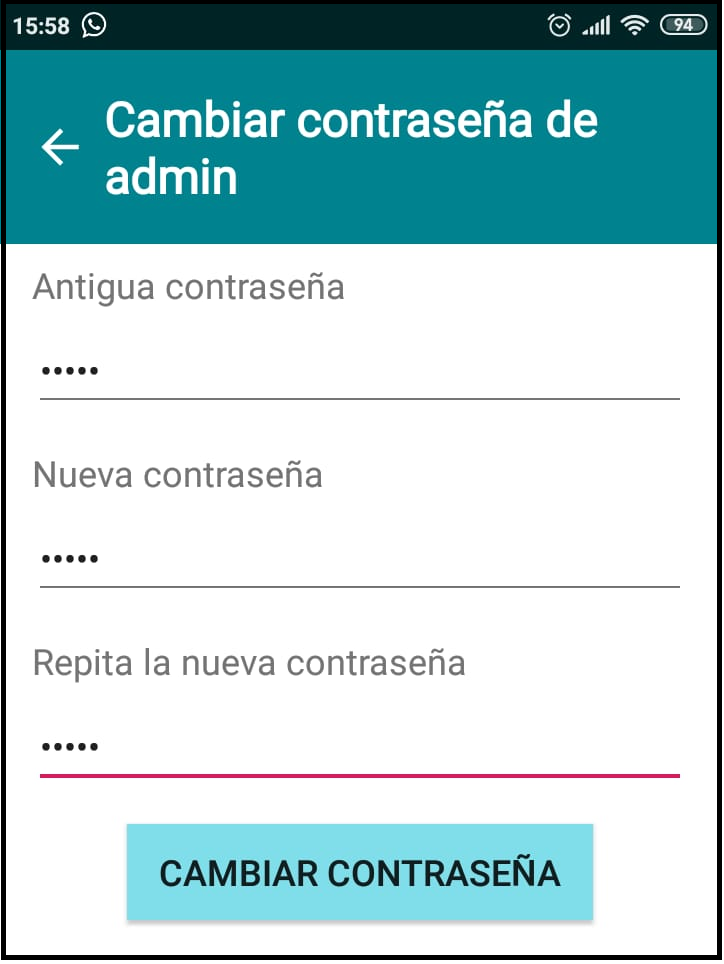
\includegraphics[width=0.35\textwidth]{../img/cambiarcontrasena.png}
	\caption{Modificar contraseña.}
	\label{fig:cambiarcontrasena}
\end{figure} 

\subsection{Acerca de}

Mediante la opción <<Acerca de>> del menú de navegación se permite acceder a una pantalla con información general sobre la aplicación, con una breve explicación de la misma, su licencia, un enlace al repositorio y la licencia de las herramientas que se han utilizado en su desarrollo. 

\begin{figure}[H]
	\centering
	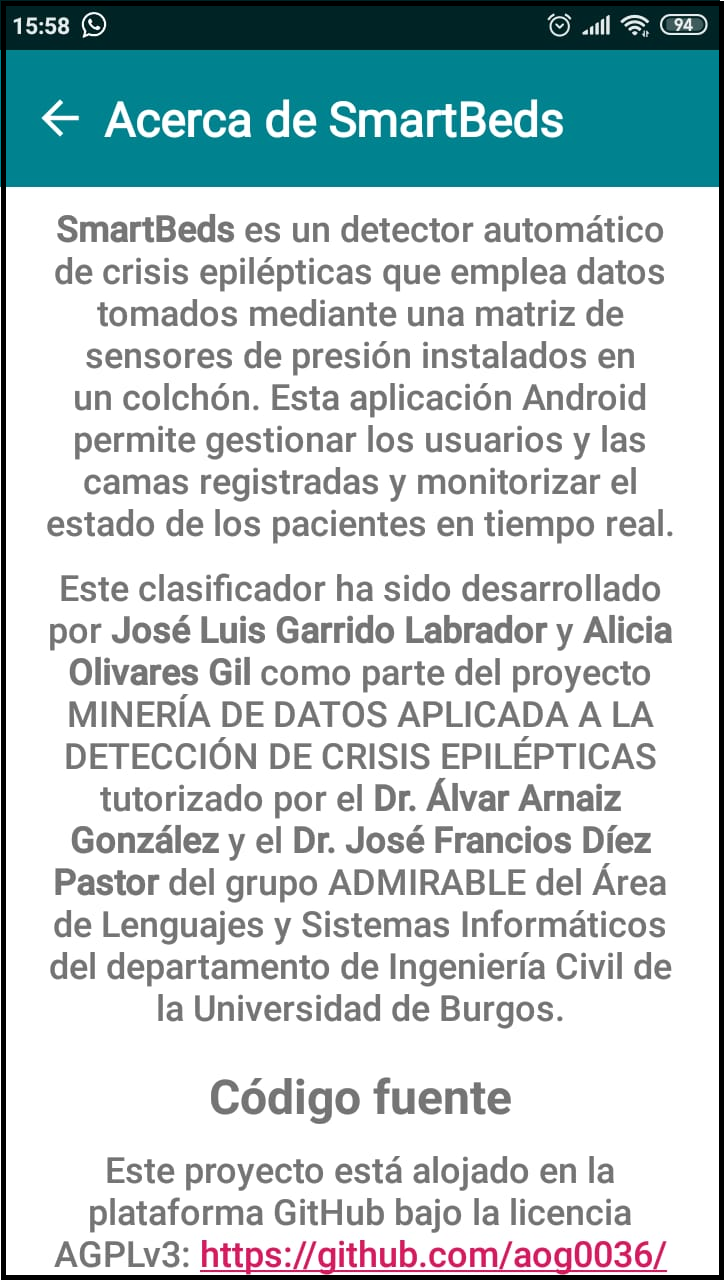
\includegraphics[width=0.35\textwidth]{../img/acercade.png}
	\caption{Acerca de la aplicación.}
	\label{fig:acercade}
\end{figure}





\bibliographystyle{plain}
\bibliography{bibliografiaAnexos}

\end{document}
